\documentclass[12pt]{report}
\usepackage{ifpdf}
%% \newif\ifpdf 
%% \ifx\pdfoutput\undefined 
%%   \pdffalse % we are not running PDFLaTeX 
%% \else 
%%   \pdfoutput=1 % we are running PDFLaTeX 
%% \pdftrue 
%% \fi
\ifpdf 
  \usepackage[pdftex]{graphicx} 
  \usepackage[pdftex]{hyperref}
  \pdfcompresslevel=9 
\else
  \usepackage{graphicx} 
  \usepackage{hyperref}
\fi
\ifpdf 
\else
\fi
\usepackage{times}
\usepackage{makeidx}
\usepackage{multirow}
\usepackage{multicol}
\usepackage{supertabular}
\author{Daren Stotler}
\title{DG manual}

\makeatletter
	\newenvironment{indentation}[3]%
	{\par\setlength{\parindent}{#3}
	\setlength{\leftmargin}{#1}       \setlength{\rightmargin}{#2}%
	\advance\linewidth -\leftmargin       \advance\linewidth -\rightmargin%
	\advance\@totalleftmargin\leftmargin  \@setpar{{\@@par}}%
	\parshape 1\@totalleftmargin \linewidth\ignorespaces}{\par}%
\makeatother 

% new LaTeX commands
\newcommand{\btwoplot}{{\bf b2plot} }


\begin{document}
\title{
\ifpdf 
  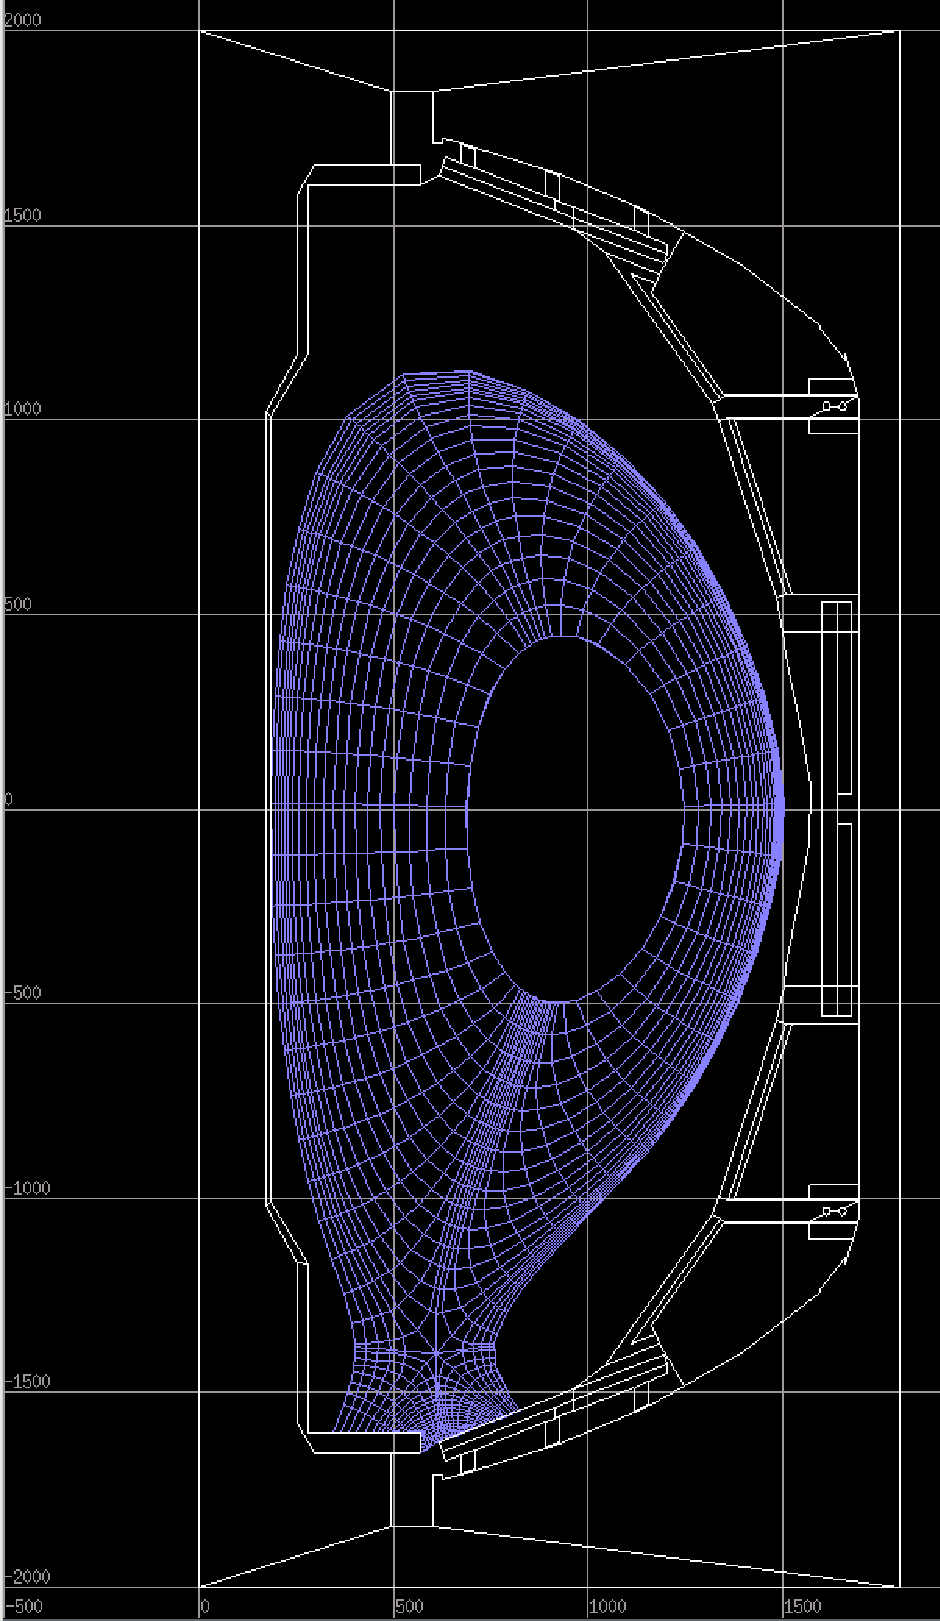
\includegraphics[height=12.0cm]{nstx_22_dg.pdf} \\
\else
  
\includegraphics[height=12.0cm]{nstx_22_dg.epsi} \\
\fi
User's Manual for DG \\
Version 2.10}
\author{Konstantin Kukushkin, Andrei Kukushkin \\
{\em ITER Organization} \\
 Alan Chin,
Daren Stotler \\
{\em Princeton Plasma Physics Laboratory}}
\begin{abstract}
This is the user's manual for the \textbf{DG} geometry definition
code. Its primary objective is to simplify the specification of the
geometry, and other input data, required for the simulation of the
boundary of magnetic fusion devices.  The most straightforward application
of the code is to divertor tokamak geometries (having one or two 
X-points), although in principle other magnetic configurations
are possible.  The flexible design of \verb!DG! allows its
output to be used with multiple magnetic fusion simulation codes,
including \verb!B2-Eirene! and \verb!DEGAS 2!.  In fact, some
of the objects defined in \verb!DG! and described in this manual
may be designed specifically for use by these codes.
\end{abstract}
\maketitle

\chapter{Introduction}

\section{Purpose of DG}

\verb!DG! is the backbone of the {\bf Interactive Graphical Interface}
package. It allows user to visualize the model geometry, to modify it,
and to specify the geometry-related data necessary for a grid
generator and modelling codes. It was originally designed to alleviate
transfer of the divertor geometry from the CAD system to the 
\verb!B2-Eirene! code package. However, it has proved to become a powerful
tool of more general purpose, allowing one, e.g., to specify
arbitrary shape of the divertor structures, to check visually the
quality of the computational grids produced by a mesh generator, to
analyse the error messages from the Monte-Carlo routine, to assess
easily the compatibility of the plasma equilibrium used in the
calculations and the wall geometry of the machine, etc. It can also
be very efficient as a sort of very simple drawing program to design
the problem geometry from scratch, and not only for \verb!B2-Eirene!. With
use of this code, the most boring and time-consuming part of the
preparatory work necessary for the edge plasma modelling in a
realistic geometry, becomes really a pleasure. Try it and see
yourself!

\section{DG objects}

\subsection{External objects}

The external objects are the files which \verb!DG! imports or exports. They
normally have default extensions by which are used by the code when
displaying the lists of files in the I/O control windows. The
following table gives a brief description of the files used in \verb!DG!.

{\raggedright
\renewcommand{\arraystretch}{1.5}
\vspace{3pt} \noindent
\begin{tabular}{|p{113pt}p{200pt}p{59pt}|}
\hline
\parbox{113pt}{\raggedright 
\textbf{Input files:}
} & {\centering 
\textbf{Description}
} & \parbox{59pt}{\centering 
\textbf{Extension}
} \\
\hline
\parbox{113pt}{\centering 
\textbf{DG model}
} & 
All the data relevant to the model
& \parbox{59pt}{\centering 
.dg
} \\
\parbox{113pt}{\centering 
\textbf{Template}
} & 
Geometry data from CAD drawing or other source
& \parbox{59pt}{\centering 
.ogr
} \\
\parbox{113pt}{\centering 
\textbf{Equilibrium}
} & 
Values of the poloidal magnetic flux on a regular grid
& \parbox{59pt}{\centering 
.equ
} \\
\parbox{113pt}{\centering 
\textbf{Mesh}
} & 
The computational grid to be used by B2-Eirene
& \parbox{59pt}{\raggedright 
~
} \\
\hline
\parbox{113pt}{\raggedright 
\textbf{Output files:}
} & 
~
& \parbox{59pt}{\raggedright 
~
} \\
\hline
\parbox{113pt}{\centering 
\textbf{DG model}
} & 
All the data relevant to the model
& \parbox{59pt}{\centering 
.dg
} \\
\parbox{113pt}{\centering 
\textbf{Output file}
} &
Specification of the \textit{elements} and some other information
\textendash{} to be used by the interface routines producing the input
files for B2-Eirene.
& \parbox{59pt}{\centering 
.dgo
} \\
\parbox{113pt}{\centering 
\textbf{Targets file}
} &
Specification of the \textit{targets} \textendash{} to be used by the
interface routines producing the input files for B2-Eirene and Sonnet / Carre.
& \parbox{59pt}{\centering 
.trg
} \\
\parbox{113pt}{\centering 
\textbf{Structure file}
} &
Specification of the structures \textendash{} to be used by the
interface routines producing the input files for Sonnet / Carre.
& \parbox{59pt}{\centering 
.str
} \\
\hline
\parbox{113pt}{\raggedright 
\textbf{Configuration file:}
} &
~
& \parbox{59pt}{\raggedright 
~
} \\
\hline
\parbox{113pt}{\raggedright 
~
} &
The file containing information on the DG \textit{layers} and
\textit{variables}.
& \parbox{59pt}{\centering 
.dgc
} \\
\hline
\end{tabular}
\vspace{2pt}

}

\subsection{Internal objects}
\label{internalobjects}

The internal objects are those with which you deal when working with
DG.

\vspace{3pt} \noindent
\renewcommand{\arraystretch}{1.5}
\begin{supertabular}{lp{300pt}}
\multicolumn{1}{c}{\textbf{Objects}}
&
\multicolumn{1}{c}{\textbf{Description}}
\\
\textbf{Drawing objects}
& 
~
\\
Points
&  
Just points (displayed as red squares) which can be used to create
\textit{elements} or for diagnostic purpose.
\\
Irregular points
&  
Every point which is not regular. A regular point connects
exactly two \textit{elements} having the same orientation (see
\textit{External normals})
\\
Elements
& 
Straight line segments (displayed in bright white) connecting
\textit{points}. Normally, they represent material surfaces
in the neutral transport code (``additional surfaces''
in \verb!Eirene! parlance). You can edit elements (create,
delete, split, join, change orientation, etc.) and assign
\textit{variables} to them.
\\
Surfaces
& 
Contours of constant poloidal flux 
(displayed
in yellow) computed from \textit{equilibrium} data. You can create,
move, and delete them. The surfaces allow you to specify the
requirements on the radial mesh for the mesh generator
(\verb!Sonnet! or \verb!Carre!), and also to
check the compatibility of your wall structures with the magnetic
configuration.
\\
Grid points
& 
Points on the separatrix which represent partition of the magnetic
surfaces in different regions for the grid generator
(\verb!Sonnet! or \verb!Carre!). They are
displayed as dashes in magenta, the separatrix being drawn in red.
\\
Separators
& 
Straight line segments (displayed in cyan) connecting the outer nodes
of the computational \textit{mesh} with surrounding \textit{structure}. The separators
also represent additional surfaces, but you can only re-position their
outer edges. Their purpose is separation of \textit{additional cells} - in
terms of \verb!Eirene!. As of V. 1.4 of \verb!DG!, ``separators'' have been temporarily 
disabled. \\
Sources             &
Special points which can be grouped together (displayed as white
asterisks). They can be used to specify the point sources of neutrals,
- and also in calculation of radiation load onto the first wall. \\
Equilibrium         &
A simple visualisation of the equilibrium data - red and blue dashes
corresponding to negative and positive, respectively, 
values of the poloidal magnetic flux. \\
Mesh                &
Computational mesh, displayed in blue, produced with a grid generator 
(\verb!Sonnet! or \verb!Carre!) and imported into \verb!DG!. 
Allows you to check the quality of the mesh and
to make the necessary corrections to the input data for the grid
generator. \\
Chords              &
Straight line segments representing the \verb!Eirene!
and \btwoplot diagnostic chords. \\
Cells               &
Regions outside the computational mesh surrounded by the elements,
separators, and the mesh edges (\textit{additional cells} - in terms of
\verb!Eirene!). \\
External normals    &
Are displayed as magenta dashes and depict the orientation of the elements. They 
point to the right as you move from the beginning to the end
of an element. This is the direction of the external normal in terms
of \verb!Eirene!. \\
Template            &
Imported graphics from external source (e.g. from CAD drawing or from
old \verb!Eirene! input file). The template is displayed in cyan, and it can
be converted into \textit{elements}. \\
Axes                &
Coordinate axes which can be displayed on the drawing. \\
Grid                &
Coordinate grid which can be displayed on the drawing. \\
X-point             & 
The X-point of the magnetic equilibrium; it effectively separates the divertor
from the core plasma.  In double-null configurations, there are two
X-points which may or may not be on the same flux surface.
The code must be told the topology of the equilibrium (see \textit{topology})
in order to locate the X-points.
This must be done before specifying \textit{surfaces} or 
\textit{grid points}.
 \\
Topology
 &  
The topology of the magnetic separatrix.  A set of commonly used topologies
is provided with \verb!DG!.  Once the \textit{equilibrium} and topology have been
imported, the code will attempt to locate the X-point(s); if successful, the
separatrix (or separatrices) will be drawn in red.
 \\
\textbf{Additional data}
 &  
~
 \\
 
Variables
 &  
Typically used to associate various pieces of data with the \textit{elements}.
This information can be then passed to 
other codes via the output files.
 \\
 
Layers
 &  
Groups of variables.
 \\
 
Targets
 &  
Bound the \textit{surfaces} in the poloidal direction, and thus must be
specified for the grid generator.  They are thus analogous to the 
actual divertor targets in a tokamak.
 \\
Structure
& 
Bound the \textit{surfaces} in the radial direction.  They are thus
analogous to the walls of the vacuum vessel in a tokamak.
\\
Target edges
&
The elements which should be reconnected to the corresponding corners
of the calculational mesh in order to avoid mismatches of the mesh and
the targets in the Monte Carlo calculations. \\
\end{supertabular}
\vspace{2pt}


\chapter{Using DG}

\section{Starting DG}

To start DG with a blank window, type:
\begin{quote}
\textbf{\texttt{dg}}
\end{quote}
at the UNIX prompt.

To start \verb!DG! with an existing model (or several models) loaded, type:
\begin{verbatim}
  ./dg <filename.dg> [...]
\end{verbatim}

After you start \verb!DG!, the main window will appear.

\section{Main window}

After you start DG, the main window appears. It has four areas: menu
bar, toolbar, work area and the message line.
% Insert screen shot?

\subsection{Menu bar}

The menu bar gives you access to the most of the DG functionality. It
contains several buttons, which can be used to open the corresponding
menus by clicking the left mouse button on it. Every menu can be torn
off and left on the screen after opening it. In order to do this, just
click at the dashed line at the top of the menu window.  In this document,
we will show menu items in \textbf{\texttt{bold typewriter}} font.

The following menus are available at present:

\begin{description}
  \item[File] You use this to start a new model, to work with
external objects (to save or open the model; to import templates,
equilibrium files, topologies, 
or computational meshes; to produce the output files
which are used for generation of the input files for computational
codes), or to quit the application.
  \item[Edit] Allows you to perform some global operations,
such as recovering from errors, selecting and de-selecting all
elements, creation or removal of groups of objects, and shift or
rotation of the picture.
  \item[View] Here you can control the overall view of the
model and specify which objects should be
visible on the screen.
  \item[Commands] Allows you to perform global commands on
the model such as converting 
a \textit{template} to \textit{elements} and 
renumbering the elements.
  \item[Variables] You will use this to specify
additional geometry-related information for the output files (eg.,
location of targets, boundary conditions for the Monte Carlo routine,
etc.).
  \item[Options] From this menu you can tailor the main window
and operating mode
to fit you preferences. It also allows you to customize the DG
variables \textit{(only for experienced users!).}
  \item[Window] Allows you to open more windows with
different views of the same model, to close the current window, to open
a window showing the statistics for the model, and to open the
\textbf{\texttt{Toolbox}}.
  \item[Help] This is the way to get some online help on DG and
to identify its current version.
\end{description}

\subsection{Toolbar}

The toolbar allows you to assign different \textit{tools} to each of
the mouse buttons. There is a separate menu for each
mouse button, each containing 
the list of available tools.

\subsection{Work area}

The work area is the area where the drawing is displayed. Here you can
move around the drawing, and you can use \textit{tools} to edit it. The
work area can optionally display coordinate axes and coordinate grid
to simplify positioning of objects.

\subsection{Message line }

The message line is located below the work area. It is used to display
error messages and information on the objects. Error messages are
sometimes displayed in an error box instead of the message line, and in
this case you must click ``OK'' to proceed.

\section{Using tools}

\textbf{Tools} are used to perform actions in the work area. They
allow you to create, move, modify, or remove objects, to query
information on the objects and to move around the drawing.
In this document, we will indicate tools in \textit{\texttt{italic
typewriter}} font.

A tool \textit{must} be assigned to a mouse button in order to be used. You can
select the tool to be assigned to each of the mouse buttons either from
the toolbar, or from the \textbf{\texttt{Toolbox}} (accessible from
the \textbf{\texttt{Window menu}}). There is one small
difference between these two options. Operating with the toolbar, 
only the left mouse button should be used to select the tools associated
with the three mouse buttons,
On the other hand, when working with the \textbf{\texttt{Toolbox}}, 
a tool is associated
with a given mouse button by clicking that button on the tool.

To use a tool, move the mouse pointer into the work area and depress
the mouse button to which the tool has been assigned. Then, you can
optionally drag the mouse. To complete the mouse drag, release the mouse button
with the mouse pointer still inside the work area. To cancel the
action associated with the drag, 
move the mouse pointer out of the work area and release the
mouse button.

Some tools require you to 'select' an object. To select an object,
move the mouse pointer to the object and depress the mouse button. The
object selected will be highlighted in another color. The
\textit{green} color means OK, while the \textit{red} one indicates
that the operation cannot be done. Normally, some explanatory text
appears in such cases on the message line.

\section{Using Undo}

You can reverse the effect of almost any operation by issuing the
\textbf{Edit \begin{math}\vert{}\end{math} Undo} menu command. You can
also reverse the effect of Undo command by
\textbf{Edit \begin{math}\vert{}\end{math} Redo}. The DG keeps track of
practically all the operations you did starting from opening the
window, and thus you can recover from almost all the errors you could
make in the coarse of the model editing. To reverse the effect of all
the Undo commands you issued, use
\textbf{Edit \begin{math}\vert{}\end{math} Redo all}.

\chapter{Working with models}
\section{Opening an existing model}

To open an existing DG model from DG, use the
\textbf{\texttt{File \begin{math}\vert{}\end{math} Open... }}menu
command. A dialog box will appear prompting you for a filename. You can
either select a file from the list or type the filename in the edit
field. Then press \textbf{\texttt{Ok}}. A new window displaying the
selected model will be opened. If you issue the
\textbf{\texttt{File \begin{math}\vert{}\end{math} Open...}} command
immediately after starting DG, the file will be loaded in the current
window. If an error happens, the error box appears. Press
\textbf{\texttt{Ok}} to close the error box.

To start DG with an existing model loaded, specify the filename on the
DG command line. If you specify multiple filenames, DG will open a
separate window for each model.

\section{Creating a new model}

\index{DG, new}
To create a new, empty model with DG, use the
\textbf{\texttt{File  \begin{math}\vert{}\end{math}  New}} menu command. A
new blank window will be opened.

When you start DG without parameters, the DG window is blank.

\section{Saving a model}

To save a model, use the
\textbf{\texttt{File  \begin{math}\vert{}\end{math}  Save...}} menu
command. A dialog box will appear prompting you for a filename. If the
current model has a filename assigned to it, this filename will appear
in the edit field. In order to save the model under a different name,
or to save the newly-created file, you should either enter the new name
in the edit field, or select a name from the list (to overwrite an
existing file). After that, press \texttt{OK}.  An autosave feature
automatically saves a version of the file with a ``\verb+~+'' 
appended to the
name every 5 minutes (see 
\textbf{\texttt{Options  \begin{math}\vert{}\end{math}  Save interval}});
of course, a new file must
be saved before this can work.  If you need to use this file (e.g.,
in the event that \verb!DG! crashes unexpectedly), you should rename this
file to remove the '\verb!~!'.

\section{Quitting DG}
\index{DG, quit}

To quit DG, you must close all windows.

To close a window, issue the
\textbf{\texttt{Window  \begin{math}\vert{}\end{math}  Close}} menu
command. You can also use the window manager to close a window
click the ``X'' at the top right of the menu. 
If you've
made changes to the model in this window, a warning box will appear.
Select \textbf{\texttt{Save}} to save the model. Select
\textbf{\texttt{Discard}} to close the window without saving changes.
Select \textbf{\texttt{Cancel}} to leave the window open.

To close all windows, use the
\textbf{\texttt{File  \begin{math}\vert{}\end{math}  Exit program}} menu
command.

There is a caveat in the current version of DG that iconified windows
containing unsaved work are not de-iconified after these commands. You
will have to de-iconify them manually in order to see their warning
boxes. All other iconified windows will be closed without problems.

\chapter{Working with elements}
\section{Converting a template}

It is often more convenient to convert a template into a set of
elements and then edit them to suit your needs, rather than to define
all elements by hand.

First, you should import the template. Choose the
\textbf{\texttt{File  \begin{math}\vert{}\end{math}  Template...}} menu
command. A dialog box will appear prompting for a filename, similar to
that for opening DG files. After importing the template, choose
\textbf{\texttt{View  \begin{math}\vert{}\end{math}  Picture view}} to
adjust the zoom factor in order to make the template visible. Enable
\textbf{\texttt{View \begin{math}\vert{}\end{math} Axes}} and
\textbf{\texttt{View \begin{math}\vert{}\end{math} Grid}} to display the
coordinate system.

DG lets you adjust the template position by moving it by a fixed
distance and/or rotating it 90 degrees around (0,0). To adjust the
position, choose the
\textbf{\texttt{Edit \begin{math}\vert{}\end{math} Move/Rotate...}} menu
command. A dialog box will appear. Enable the
\textbf{\texttt{Template}} check box. To move the template, enter X-
and Y-increments and press \textbf{\texttt{Move}}. To rotate, press
\textbf{\texttt{Rotate}}. If the template moves out of sight, again
choose \textbf{\texttt{View \begin{math}\vert{}\end{math} Picture view}}.
Press \textbf{\texttt{Close}} when done.

To convert the template into a set of elements, choose
\textbf{\texttt{Commands \begin{math}\vert{}\end{math} Convert
template}}.

Note that after the conversion, the template remains visible. This is
convenient for editing elements, because the difference from the
original template is visible. You can hide or display the template by
disabling or enabling
\textbf{\texttt{View \begin{math}\vert{}\end{math} Template}}. To unload
the template permanently, choose
\textbf{\texttt{Edit \begin{math}\vert{}\end{math} Delete \begin{math}\vert{}\end{math} Template}}.

Elements produced in this manner are sometimes improperly connected or
have wrong external normals. Manual editing of the elements may be required to 
remedy these problems. 

\section{Creating elements manually}

There are several tools for creating new elements.

Use \textit{\texttt{Add element}} to create the first element or to
attach an element to a pre-defined point. Move the mouse pointer to the
starting point and press the mouse button. Then move the pointer to the
ending point and release the mouse button.

Use \textit{\texttt{Split element}} to split an element into two.
Select an element. It will split into two. Drag the newly created point
to the desired location and release the mouse button.

Use \textit{\texttt{Connect points}} to create an element between two
predefined points. Select the first point, move the mouse cursor to
the second one and release the mouse button. You cannot create more
than one element between the same two points.

You can also use the
\textbf{\texttt{Edit  \begin{math}\vert{}\end{math}  Create \begin{math}\vert{}\end{math}  Point...}}
menu command to create points that will be later connected using the
\textit{\texttt{Connect points}} tool. A dialog box will appear. Enter
the desired coordinates and press \textbf{\texttt{Create}}. The dialog
box will remain on the screen, allowing you to create more than one
point without reopening it. To close the dialog box, press Cancel.

\section{Editing elements}

There are several tools for modifying existing elements.

Use \textit{\texttt{Delete }}to remove an element. Select the element
and release the mouse button. Deleting all of the elements connected
to a given point also deletes that point.

Use \textit{\texttt{Join elements}} to join two adjanced elements into
one (reverse effect of \textit{\texttt{Split element}}). Select the
point between the elements and release the mouse button. You can only
join elements around a regular point. There must be exactly two
elements attached and their external normals must point to the same
direction.

Use \textit{\texttt{Move}} to move a point with all attached
elements. Select the point and drag it to the new location. Then
release the mouse button.

Use \textit{\texttt{Reposition}} to attach one end of an element to
another point. Select the element near one of its ends, move the mouse
pointer to another pre-defined point and release the button.

\section{Changing external normals}

Having the external normals of adjacent elements aligned permits them
to be easily marked; some operations also require the normals of
adjacent elements to be aligned (i.e., for the points involved in the
operation to 
all be regular). 

To display or hide external normals, enable or disable
\textbf{\texttt{View  \begin{math}\vert{}\end{math}  External normals}}.

Use the \textit{\texttt{Reverse normals}} tool to change directions of
external normals. Select an element to change its normal. Moving the
mouse pointer to adjacent elements will force their normals to point to
the same direction as that of the first element. Release the mouse
button to end the action.

\section{Renumbering elements}

Each element has a integer label associated with it. These
determine the order in which the elements are written 
into the output file. This
feature is very useful for debugging. DG uses an internal counter to
assign these numbers. Each time the user creates an element, the
counter is incremented by one and its value is used as the element
number. However, when the user deletes an element, the remaining elements are
not renumbered and the counter is not decremented. Since many unused
numbers consume disk space and may slow down programs that use DG
output, these unused element numbers should be periodically eliminated.
Renumbering elements is
absolutely safe except when you are doing some debugging and need these
numbers to identify elements in the output file.

To display or hide element numbers, enable or disable
\textbf{\texttt{View  \begin{math}\vert{}\end{math}  Display  \begin{math}\vert{}\end{math}  Numbers}}.

To count unused numbers, choose
\textbf{\texttt{Window  \begin{math}\vert{}\end{math}  Statistics}} in order
to display information about the current file. The 'unused numbers'
entry contains this count.

To eliminate unused element numbers, choose
\textbf{\texttt{Commands  \begin{math}\vert{}\end{math}  Renumber
elements}}.

\chapter{Controlling how objects are displayed}

\section{Changing the zoom factor and location}

You can use the \textit{\texttt{Zoom}} tool to move around the drawing
and to change the zoom factor. You can also use commands from the
\textbf{\texttt{View}} menu.

To move around with the \textit{\texttt{Zoom}} tool, press and release
the mouse button anywhere in the work area without moving the mouse.
The work area will be adjusted so that the location where the button
was pressed is moved to the center. Alternatively, you can press
Shift+mouse button, move the mouse pointer and release the button. The
work area will be adjusted so that the location where the button was
pressed is now shown where the button has been released.

To change the zoom factor with the \textit{\texttt{Zoom}} tool, press
the mouse button, move the mouse in order to draw a rectangle around
the area to be shown in the work area. Then, release the mouse button.
Note that the area actually shown may be enlargened in order to
preserve the aspect ratio.

The \textbf{\texttt{View \begin{math}\vert{}\end{math} Zoom in}} command
increases the zoom factor.

The \textbf{\texttt{View \begin{math}\vert{}\end{math} Zoom out}}
command decreases the zoom factor.

The \textbf{\texttt{View \begin{math}\vert{}\end{math} Picture view}}
command adjusts the zoom factor and location so that all objects fit
into the work area. This command ignores objects that are hidden
because of settings in the \textbf{\texttt{View}} menu.

The \textbf{\texttt{View \begin{math}\vert{}\end{math} Selection view}}
command adjusts the zoom factor and location so that all marked objects
fit into the work area.

\section{Hiding and displaying objects}

Toggle buttons in the \textbf{\texttt{View}} menu let you hide or
display the coordinate system and various kinds of objects.

Note that you cannot select an object that is not displayed. In
particular, you can only select points that are displayed (a small
square is drawn around the point). The
\textbf{\texttt{View \begin{math}\vert{}\end{math} Points}} setting
controls the display of points. When it is disabled, the
\textbf{\texttt{View \begin{math}\vert{}\end{math} Irregular points}}
setting controls the display of irregular points. It is convenient to
display only irregular points while correcting a converted template,
because irregularities can be seen very easily.

\section{Rotating the view}
\label{rotateview}

The display may now be viewed at any angle of rotation. The user may
specify the desired angle by using the 
Rotate tool, the commands under the 
\textbf{\texttt{View  \begin{math}\vert{}\end{math}  Rotate}} menu,
or the equivalent 
keyboard shortcuts to increment (``Ctrl+(''), decrement (``Ctrl+)''), or
zero the angle (\textbf{\texttt{Rectify}}, 
shortcut ``Ctrl+C''); see Fig.~\ref{rotate30}. 
The rotation does not affect the
underlying structures being displayed, but only the drawing procedure.
The \textbf{\texttt{Previous view}} command will undo rotations.
Rotations are saved starting with file format version 115.  
Files of older formats are still compatible; the default angle will be 0.
Note that the Picture View command 
(\textbf{\texttt{View  \begin{math}\vert{}\end{math}  Picture View}}) zeroes
the rotation angle.

\begin{figure}
\ifpdf
  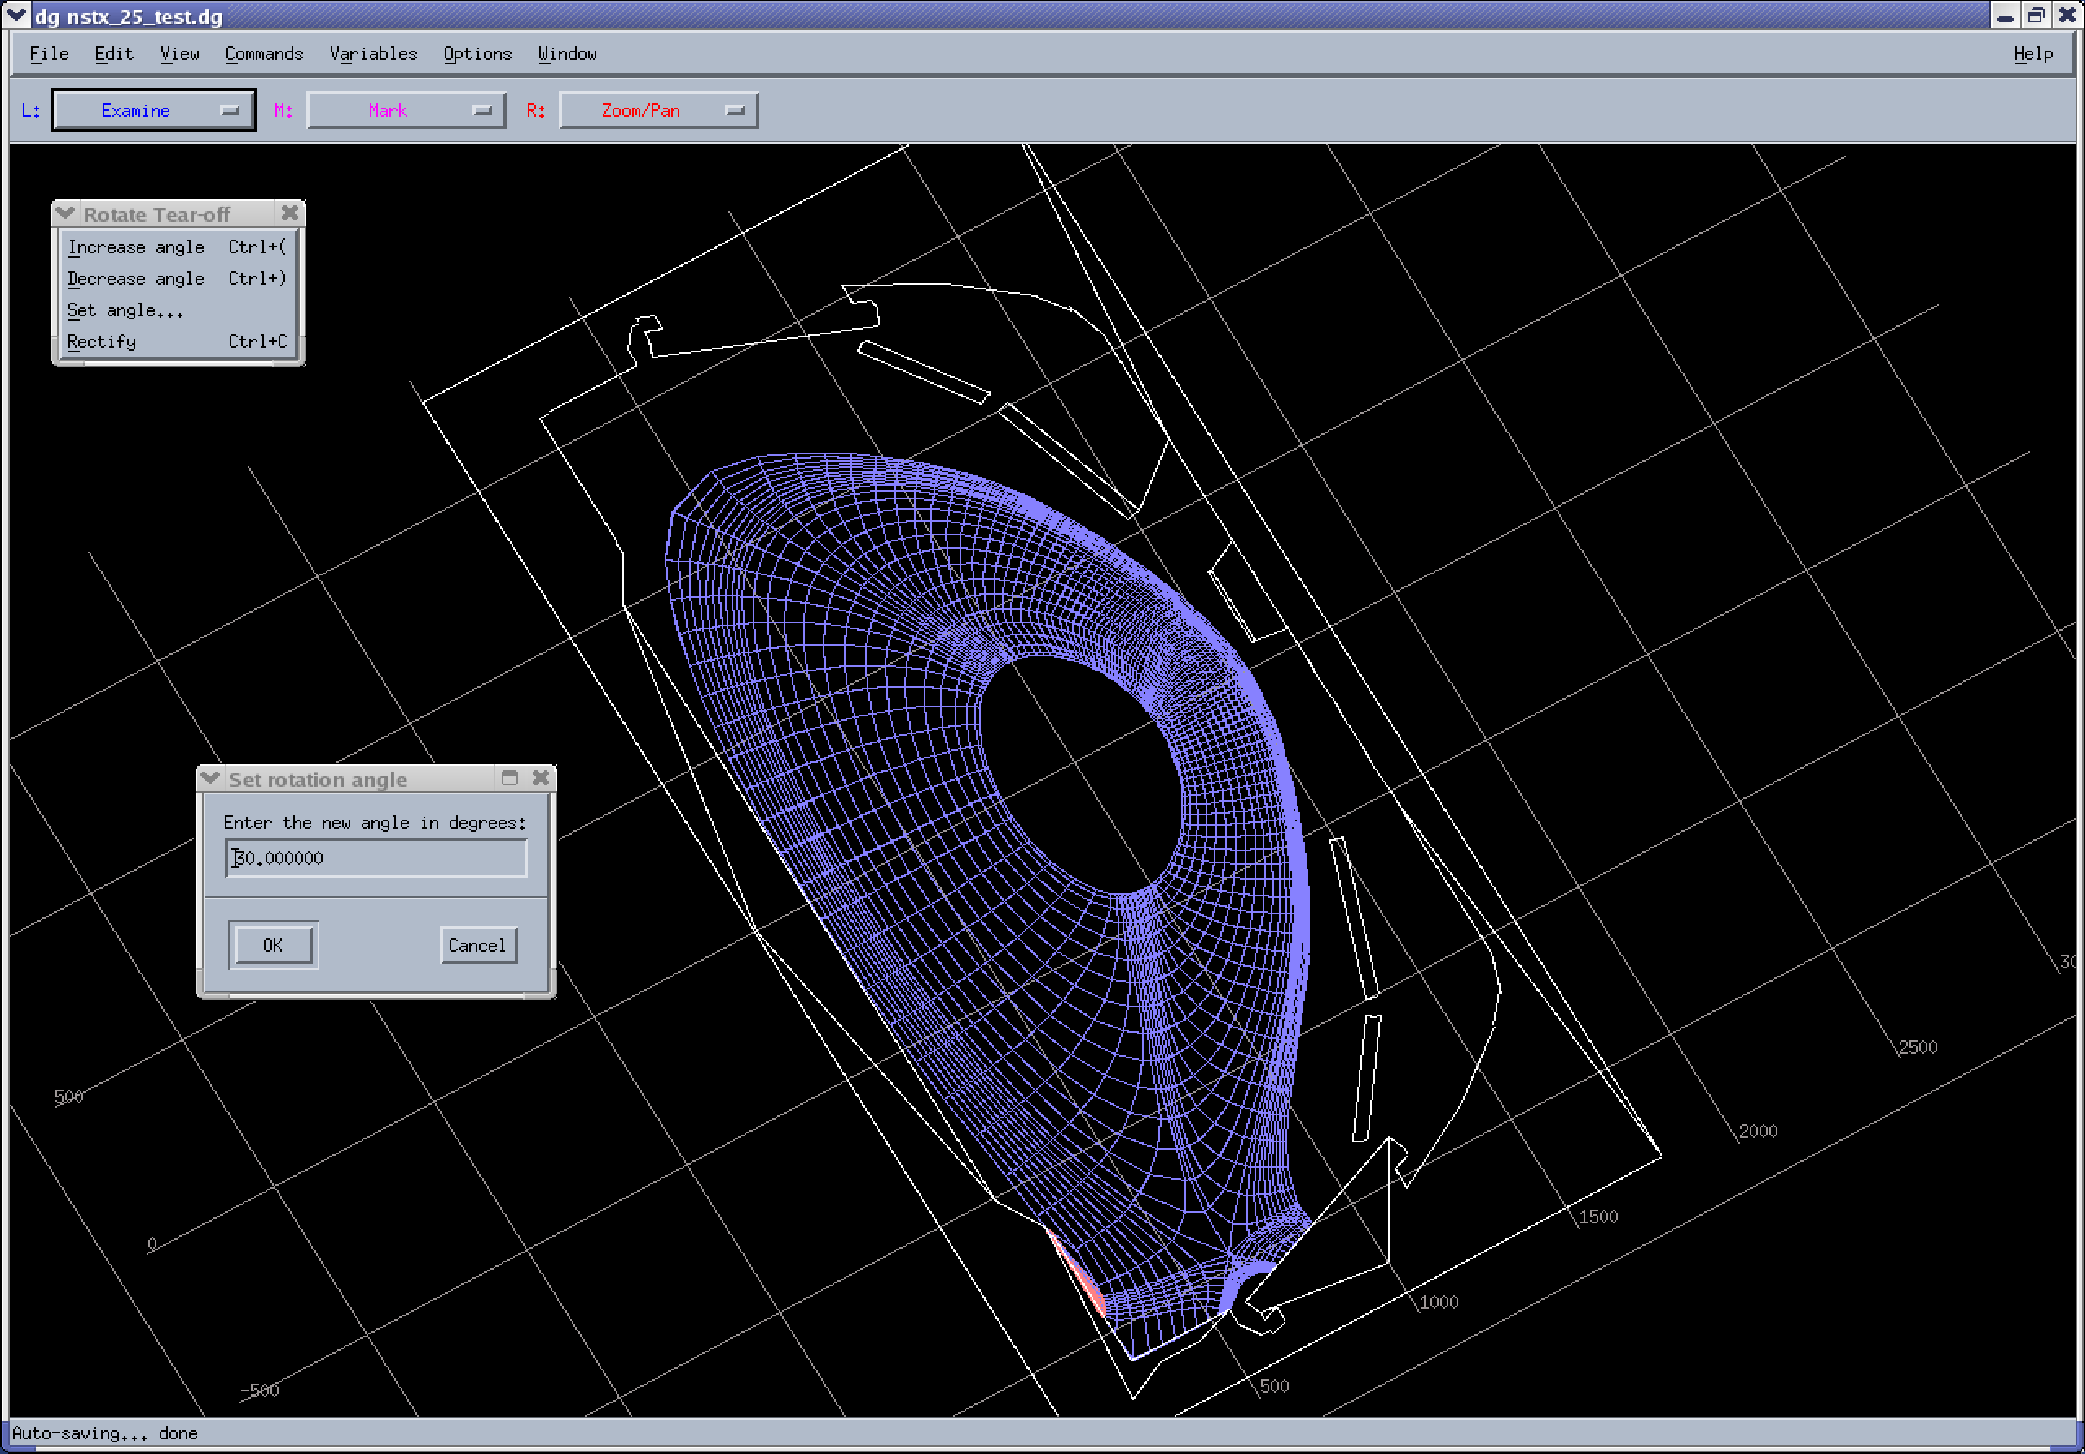
\includegraphics[width=15.0cm]{rotation_30.pdf}
\else
  
\includegraphics[width=15.0cm]{rotation_30.epsi}
\if
\caption{Demonstration of a rotated view with associated dialog box and
tear-off menu.}
\label{rotate30}
\end{figure}

\section{Stretching and shrinking the view}
\label{stretchview}

The aspect ratio may be ``unlocked'' by enabling the 
\textbf{\texttt{View  \begin{math}\vert{}\end{math}  Mode  \begin{math}\vert{}\end{math}  Stretch}} button.
In Stretch view mode, the
\textbf{\texttt{View  \begin{math}\vert{}\end{math}  Stretch/Shrink}}
menu item becomes active (see Fig.~\ref{stretch2x5y}), 
and the user may use these tools to
stretch or shrink the $x$ and $y$ axes. 
To stretch or shrink the current view by a factor of 2, 
use the first four buttons of this menu.  The keyboard shortcuts are
``Ctrl+Shift+H'' to stretch horizontally (in the $x$ direction), 
``Ctrl+H'' to shrink horizontally, ``Ctrl+Shift+V'' to stretch vertically
(in the $y$ direction), and ``Ctrl+V'' to shrink vertically.  
Precise stretching or shrinking factors can be specified with the
\textbf{\texttt{Stretch\ldots}} dialog.  The aspect ratio can be reset
with the \textbf{\texttt{Justify}} menu item.
Additionally, zooming with the highlighted
rectangle now zooms to display exactly the contents inside the rectangle,
rather than expanding to ensure the proper aspect ratio. Disabling
Stretch mode redraws the display with proper aspect ratio and
preserves the ratio in future changes of view.

\begin{figure}
\ifpdf
  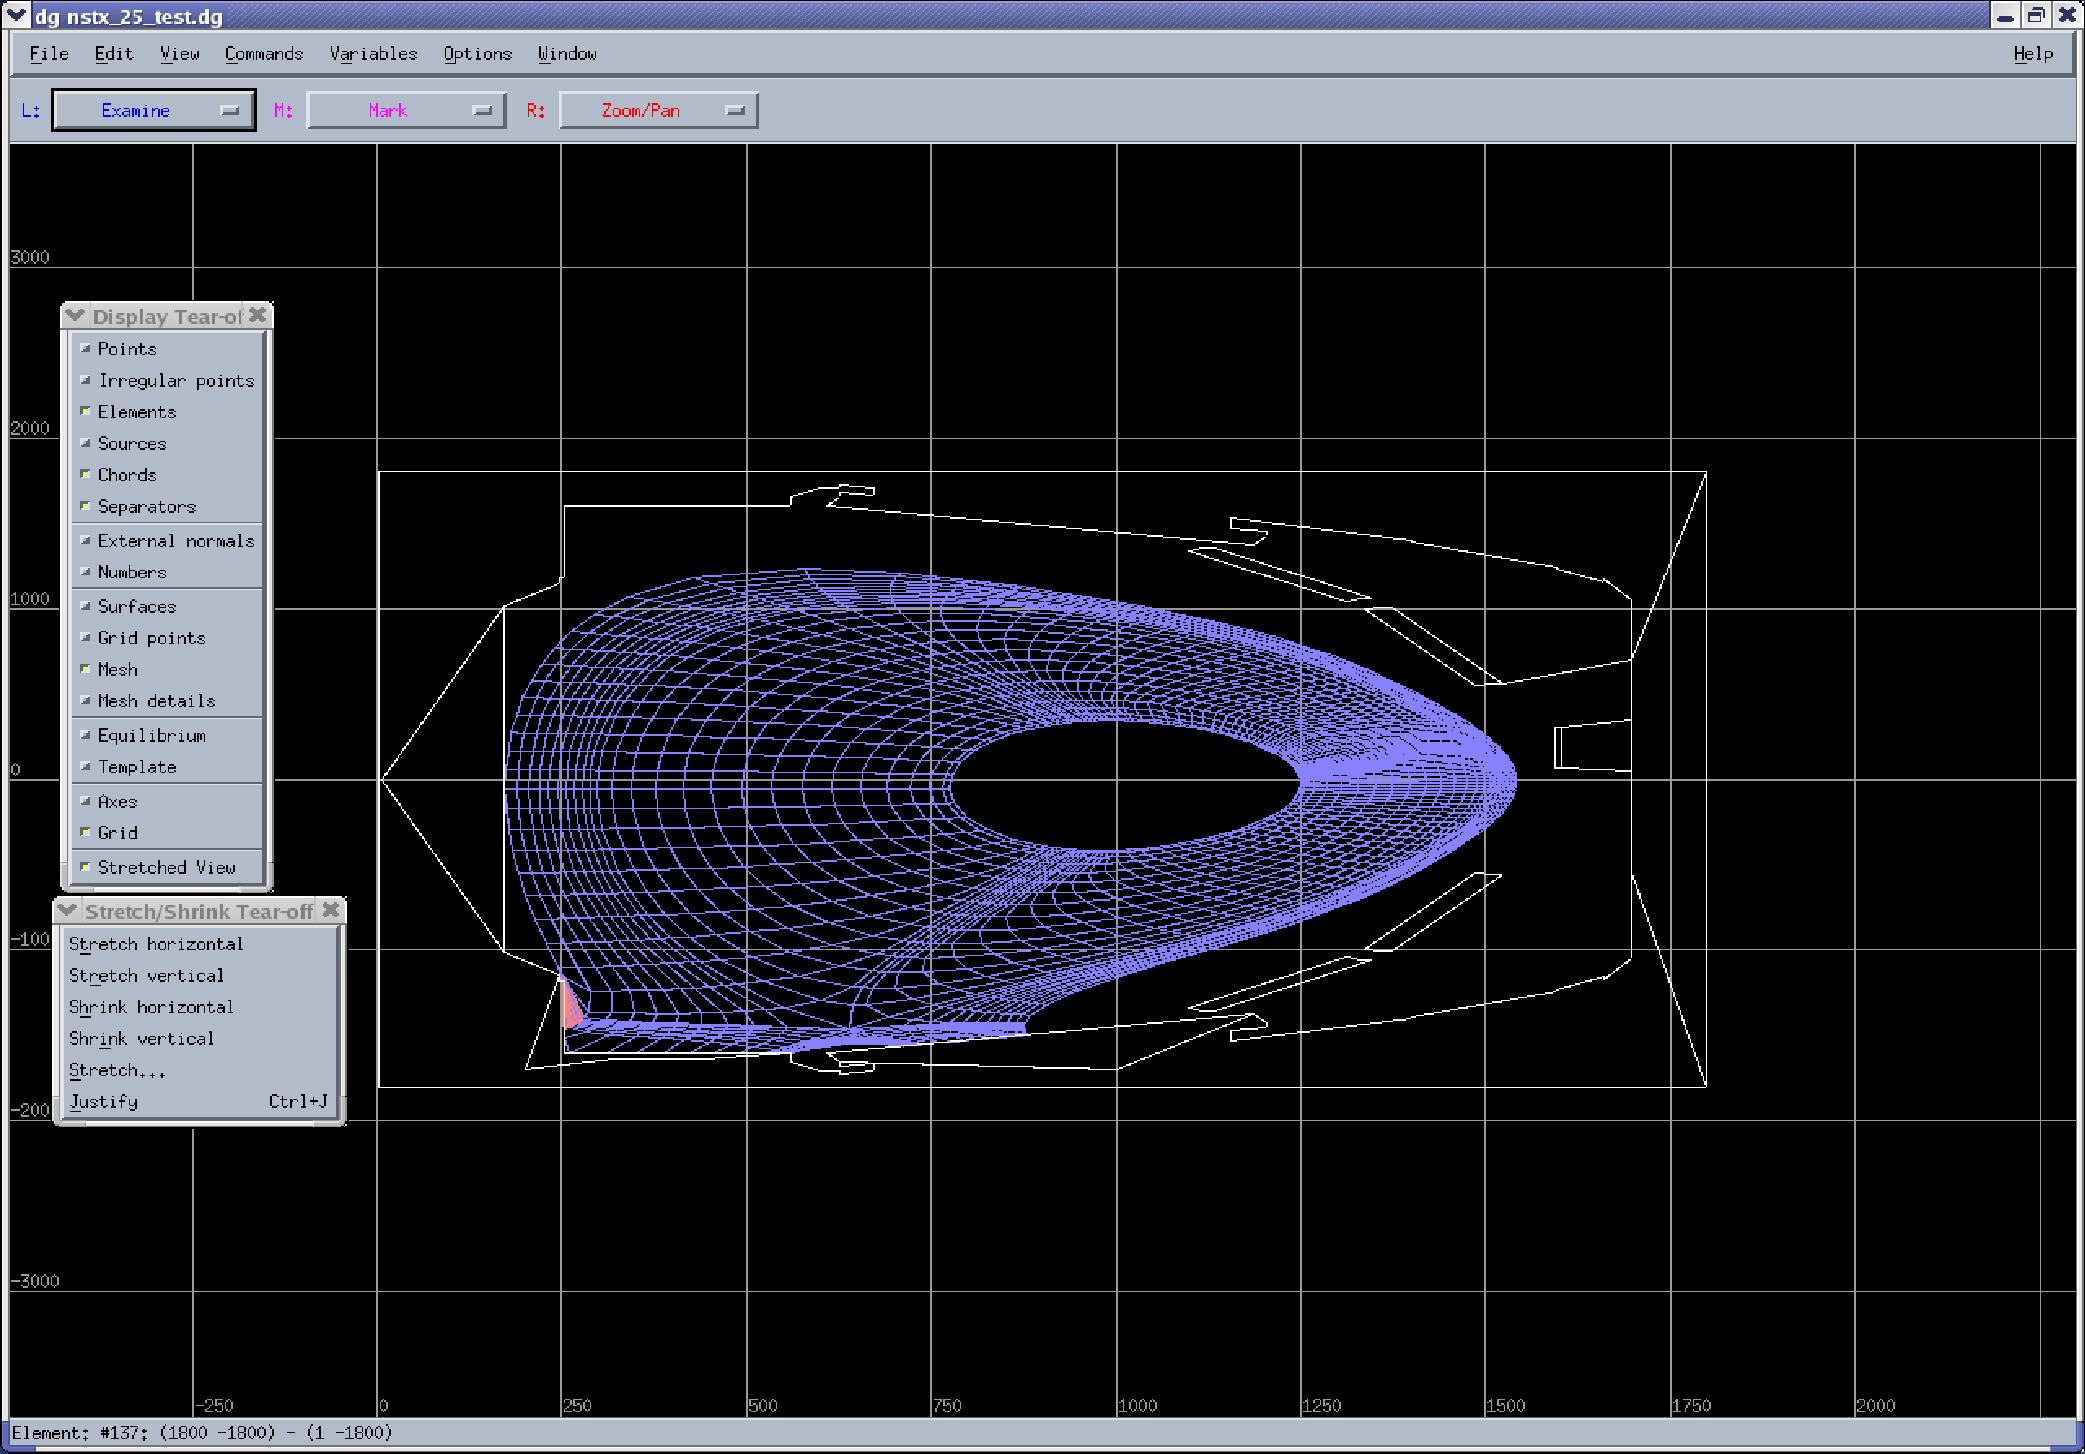
\includegraphics[width=15.0cm]{stretch_2x_5y.pdf}
\else
  
\includegraphics[width=15.0cm]{stretch_2x_5y.epsi}
\fi
\caption{Demonstration of the variable aspect ratio capability along with
the associated tear-off menu.}
\label{stretch2x5y}
\end{figure}

The \textit{\texttt{Stretch}} 
tool works a little differently since it can stretch either
horizontally or vertically.  If the mouse is within 45$^{\circ}$ of an
imaginary horizontal line through the center of the window, a mouse drag
will stretch or shrink the view in the horizontal direction.  Likewise, if the
mouse is within 45$^{\circ}$ of the vertical line through the center of
the window, a mouse drag stretches or shrinks in the veritical 
direction.  If \textbf{\texttt{Stretch mode}} 
is disabled, the \textit{\texttt{Stretch}} tool does
nothing.

Note that the Picture View command 
(\textbf{\texttt{View  \begin{math}\vert{}\end{math}  Picture View}}) resets
the aspect ratio, but does not disable Stretch mode.


% We still have Alan's description of the application of the stretch and
% rotation capability to manipulate mesh cells. Suggest putting it later
% with mesh related stuff or perhaps in an appendix.
\section{Top-down view}
\label{topdownview}

To facilitate visualization and specification of Chords 
with nonzero toroidal extent (see Ch.~\ref{chords}), a view from above the
torus is now available via the
\textbf{\texttt{View  \begin{math}\vert{}\end{math}  Mode  \begin{math}\vert{}\end{math}  Top-down view}}
button.  When this button is enabled, the main window depicts the view of the
present geometry looking down along the $y$ axis.  The elements in the
model are assumed to be toroidally symmetric.  In this view, the elements are
displayed as 48 (arbitrarily chosen) straight line segments.  The only
other objects currently displayed in this view are chords, although
working drawing procedures exist for all markable objects. Since displaying
every element in the model would likely result in confusion, the user
must select the specific elements to be depicted.  The variable
\textbf{\texttt{Top View Elements}} has been defined for this purpose
(\textbf{\texttt{Variables  \begin{math}\vert{}\end{math}  Top View Elements}}).
The appearance of chords (with some toroidal extent) can be toggled with
either \textbf{\texttt{View  \begin{math}\vert{}\end{math}  Display  \begin{math}\vert{}\end{math}  Chords}} 
or \textbf{\texttt{View  \begin{math}\vert{}\end{math}  Display  \begin{math}\vert{}\end{math}  3dchords}}.
As in the normal (poloidal) view, 
\textbf{\texttt{View  \begin{math}\vert{}\end{math}  Display  \begin{math}\vert{}\end{math}  Elements}} toggles the appearance of elements in the top view.
Since top view was intended to be used only for chords, many tools are 
disabled in this mode.  Likewise, since top view uses the same 
screen coordinates as the normal view, it may be necessary to rezoom 
after switching between the two views.  
\textbf{\texttt{View  \begin{math}\vert{}\end{math}  Picture View}}
can be used for this purpose in either mode. 

\chapter{Working with magnetic surfaces and grid points}

\section{Equilibrium conversion and manipulation}
\label{equtrn}

The \texttt{DG/equtrn} 
directory has some utilities for converting between various
widely used formats for magnetic equilibrium files and for making minor
modifications to them.

\subsection{d2d}

This is a script that invokes the \textbf{\texttt{dg2dg}} executable.  Its sole
function is to double the resolution of a DG equilibrium file.  To 
invoke it:
\begin{quote}
\textbf{\texttt{d2d $<$filein$>$.equ $<$fileout$>$.equ}}
\end{quote}
\subsection{d2e}

This is a script that invokes the \textbf{\texttt{dg2ef}} 
executable to convert a
DG equilibrium file to the EFIT format (specifically, the EFIT ``g'' file).
This is invoked with (the file suffixes are recommended for clarity
and are not enforced):
\begin{quote}
\textbf{\texttt{d2e $<$filein$>$.equ $<$fileout$>$.efit}}
\end{quote}
Some older DG files lack the magnetic field data needed for this conversion.
The default name for the file containing its value is 
\textbf{\texttt{field.snn}} (i.e., using the above invocation).  
Alternatively, the name of the file containing the field can be 
specified as a third argument:
\begin{quote}
\textbf{\texttt{d2e $<$filein$>$.equ $<$fileout$>$.efit $<$fieldfile$>$}}
\end{quote}
\subsection{d2v}

This is a script that invokes the \textbf{\texttt{dg2vr}} 
executable to convert a
DG equilibrium file to the Carre (or TdeV) equilibrium 
format.
This is invoked with (the file suffixes are recommended for clarity
and are not enforced):
\begin{quote}
\textbf{\texttt{d2v $<$filein$>$.equ $<$fileout$>$.v}}
\end{quote}
Some older DG files lack the magnetic field data needed for this conversion.
The default name for the file containing its value is 
\textbf{\texttt{field.snn}} (i.e., using the above invocation).  
Alternatively, the name of the file containing the field can be 
specified as a third argument:
\begin{quote}
\textbf{\texttt{d2v $<$filein$>$.equ $<$fileout$>$.v $<$fieldfile$>$}}
\end{quote}
\subsection{e2d}

This is a script that invokes the \textbf{\texttt{ef2dg}} 
executable to convert an EFIT format (specifically, the EFIT ``g'' file)
equilibrium to the format read by DG. 
This is invoked with (the file suffixes are recommended for clarity
and are not enforced):
\begin{quote}
\textbf{\texttt{e2d $<$filein$>$.efit $<$fileout$>$.equ}}
\end{quote}
\subsection{n2d}

This is a script that invokes the \textbf{\texttt{nk2dg}} 
executable to convert an equilibrium in the
``Naka'' format
to the format read by DG. 
This is invoked with (the file suffixes are suggested for clarity
and are not enforced):
\begin{quote}
\textbf{\texttt{e2d $<$filein$>$.nk $<$fileout$>$.equ}}
\end{quote}
\subsection{rps}

This is a script that invokes the \textbf{\texttt{risepsi}} executable. 
Its sole
function is to increase the poloidal flux values in the
DG equilibrium file by the specified amount.  To 
invoke it:
\begin{quote}
\textbf{\texttt{rps $<$filein$>$.equ $<$fileout$>$.equ $<$increment$>$}}
\end{quote}
\subsection{v2d}

This is a script that invokes the \textbf{\texttt{vr2dg}} 
executable to convert an equilibrium in the Carre (or TdeV) format
to the format read by DG. 
This is invoked with (the file suffixes are recommended for clarity
and are not enforced):
\begin{quote}
\textbf{\texttt{v2d $<$filein$>$.v $<$fileout$>$.equ}}
\end{quote}
By default, this script will look for the value of the magnetic field
in a file \textbf{\texttt{field.snn}}. 
Alternatively, the name of the file containing the field can be 
specified as a third argument:
\begin{quote}
\textbf{\texttt{v2d $<$filein$>$.v $<$fileout$>$.equ $<$fieldfile$>$}}
\end{quote}
\subsection{cropequ}

This is an executable (no corresponding script) that crops a
DG equilibrium file.  The code is invoked with:
(the file suffixes are recommended for clarity
and are not enforced):
\begin{quote}
\textbf{\texttt{cropequ $<$filein$>$.equ $<$fileout$>$.equ}}
\end{quote}
The code will print out the dimension and spatial extent of the input
equilibrium grid then request the values for the output grid in the
order: number of radial grid points, minimum radius, maximum radius,
number of vertical grid points, minimum vertical coordinate, 
maximum vertical coordinate.  The maximum number of grid points is 257
(can be increased via a parameter statement in the code).  The code
will requires the requested spatial extent to lie within that of the
input grid.  If it does not, the offending parameter is reset to
match the corresponding value from the input grid.

\subsection{prinequ}

This is an executable (no corresponding script) that prints out the
contents of a DG equilibrium file in tabular format.  The file 
is read from standard input and the result is sent to standard out.
So, the preferred invocation would be
(the file suffixes are recommended for clarity
and are not enforced):
\begin{quote}
\textbf{\texttt{prinequ $<$ $<$filein$>$.equ $>$ $<$fileout$>$.txt}}
\end{quote}

\section{Importing equilibrium}

An equilibrium file must be imported before defining any surfaces or
grid points.

To import an equilibrium file, choose
\textbf{\texttt{File $\mid$ Import $\mid$ Equilibrium...}} . A
dialog box will appear prompting for a filename. Select a file and
press \textbf{\texttt{Ok}}. Select
\textbf{\texttt{View \begin{math}\vert{}\end{math} Picture view}} to make
sure the equilibrium grid is visible in the work area. Red color
represents positive  \begin{math}\psi{}\end{math}  values, while blue
represents the negative ones.

\section{Output mode}

The detailed procedures for creating and editing surfaces and grid
points differ slightly for the Sonnet and Carre mesh generators.
So, before undertaking these tasks, the user should select the
appopriate output mode in \textbf{\texttt{Options $\mid$ Output mode}}.
Since only the Carre code is distributed along with this manual,
only procedures pertinent to it will be described.

This dialog box also allows the user to determine which objects are
examined for consistency when DG's output is requested
(via \textbf{\texttt{File $\mid$ Output...}}).  Selecting all of these
checks is recommended.  Users should override them only if they are
aware of the consequences of the object in question being improperly
defined.

\section{Creating and editing surfaces}
\label{createsurfaces}

As was noted in Sec.~\ref{internalobjects}, surfaces are drawn between
targets and are bounded by structures.  
The target related variables are single elements set using the
variables 
\textbf{\texttt{Variables $\mid$ Inner edge of inner target}}, etc.,
where the first ``inner'' and ``outer'' refers to the inner and outer edge
of the computational mesh, respectively, and the second to the
usual inner and outer divertor target.  There is an additional
set of targets available for double null geometries; see:
\textbf{\texttt{Variables $\mid$ Add $\mid$ Extra targets for DN}}.
The structures are set with the variable
\textbf{\texttt{Variables $\mid$ Structure}}.  There may be one or more
of these.

In Carre mode, the user begins the process of surface creation by manually
creating the surface that will represent the innermost core surface
via the \textit{\texttt{Add surface}} tool.  
Just click it inside core plasma at the
desired location (the tool will not work anywhere else).
Its location can be altered via the \textit{\texttt{Move}}
tool.  It can only be deleted
by executing the \textbf{\texttt{Edit $\mid$ Delete $\mid$ Surfaces}} command
(this deletes {\em all} surfaces).

The next step is to open the \textbf{\texttt{Create surface(s)...}} dialog,
\textbf{\texttt{Edit  \begin{math}\vert{}\end{math}  Create \begin{math}\vert{}\end{math}  Surfaces...}} (see Fig~\ref{createsurfacesfig}).
In Carre mode, the user can only create multiple surfaces (i.e., the ``Single''
option will not work).  The ''Area'' menu determines in which part
(topologically) of the equilibrium the surfaces will be drawn.  The number
of Cells must be input manually.  The line graph in the dialog box is a
simple depiction of the relative spacing of the surfaces.  In Carre mode,
only the ``Delta Law'' is available.  In this case, the two parameters
``Delta1'' and ``Delta2'' specify a quadratic function used to determine
this spacing  
(The deltas specify the relative normalized
difference between the levels of the
first two, and the last two surfaces).

While these parameters can be input directly, the preferred
means of setting them is to click and drag the black line in the graph to
achieve the desired spacing variation.  When the ``Create'' button is
clicked, the surfaces will be generated with this spacing and drawn in 
DG's main window.  If a model has an existing set of surfaces that the
user wishes to tweak, click on one with the \textit{\texttt{Examine}} tool and then
click the ``\verb+<<+'' button in the \textbf{\texttt{Create surface(s)...}} 
dialog; this will
import the parameters describing these surfaces.

\begin{figure}
\ifpdf
  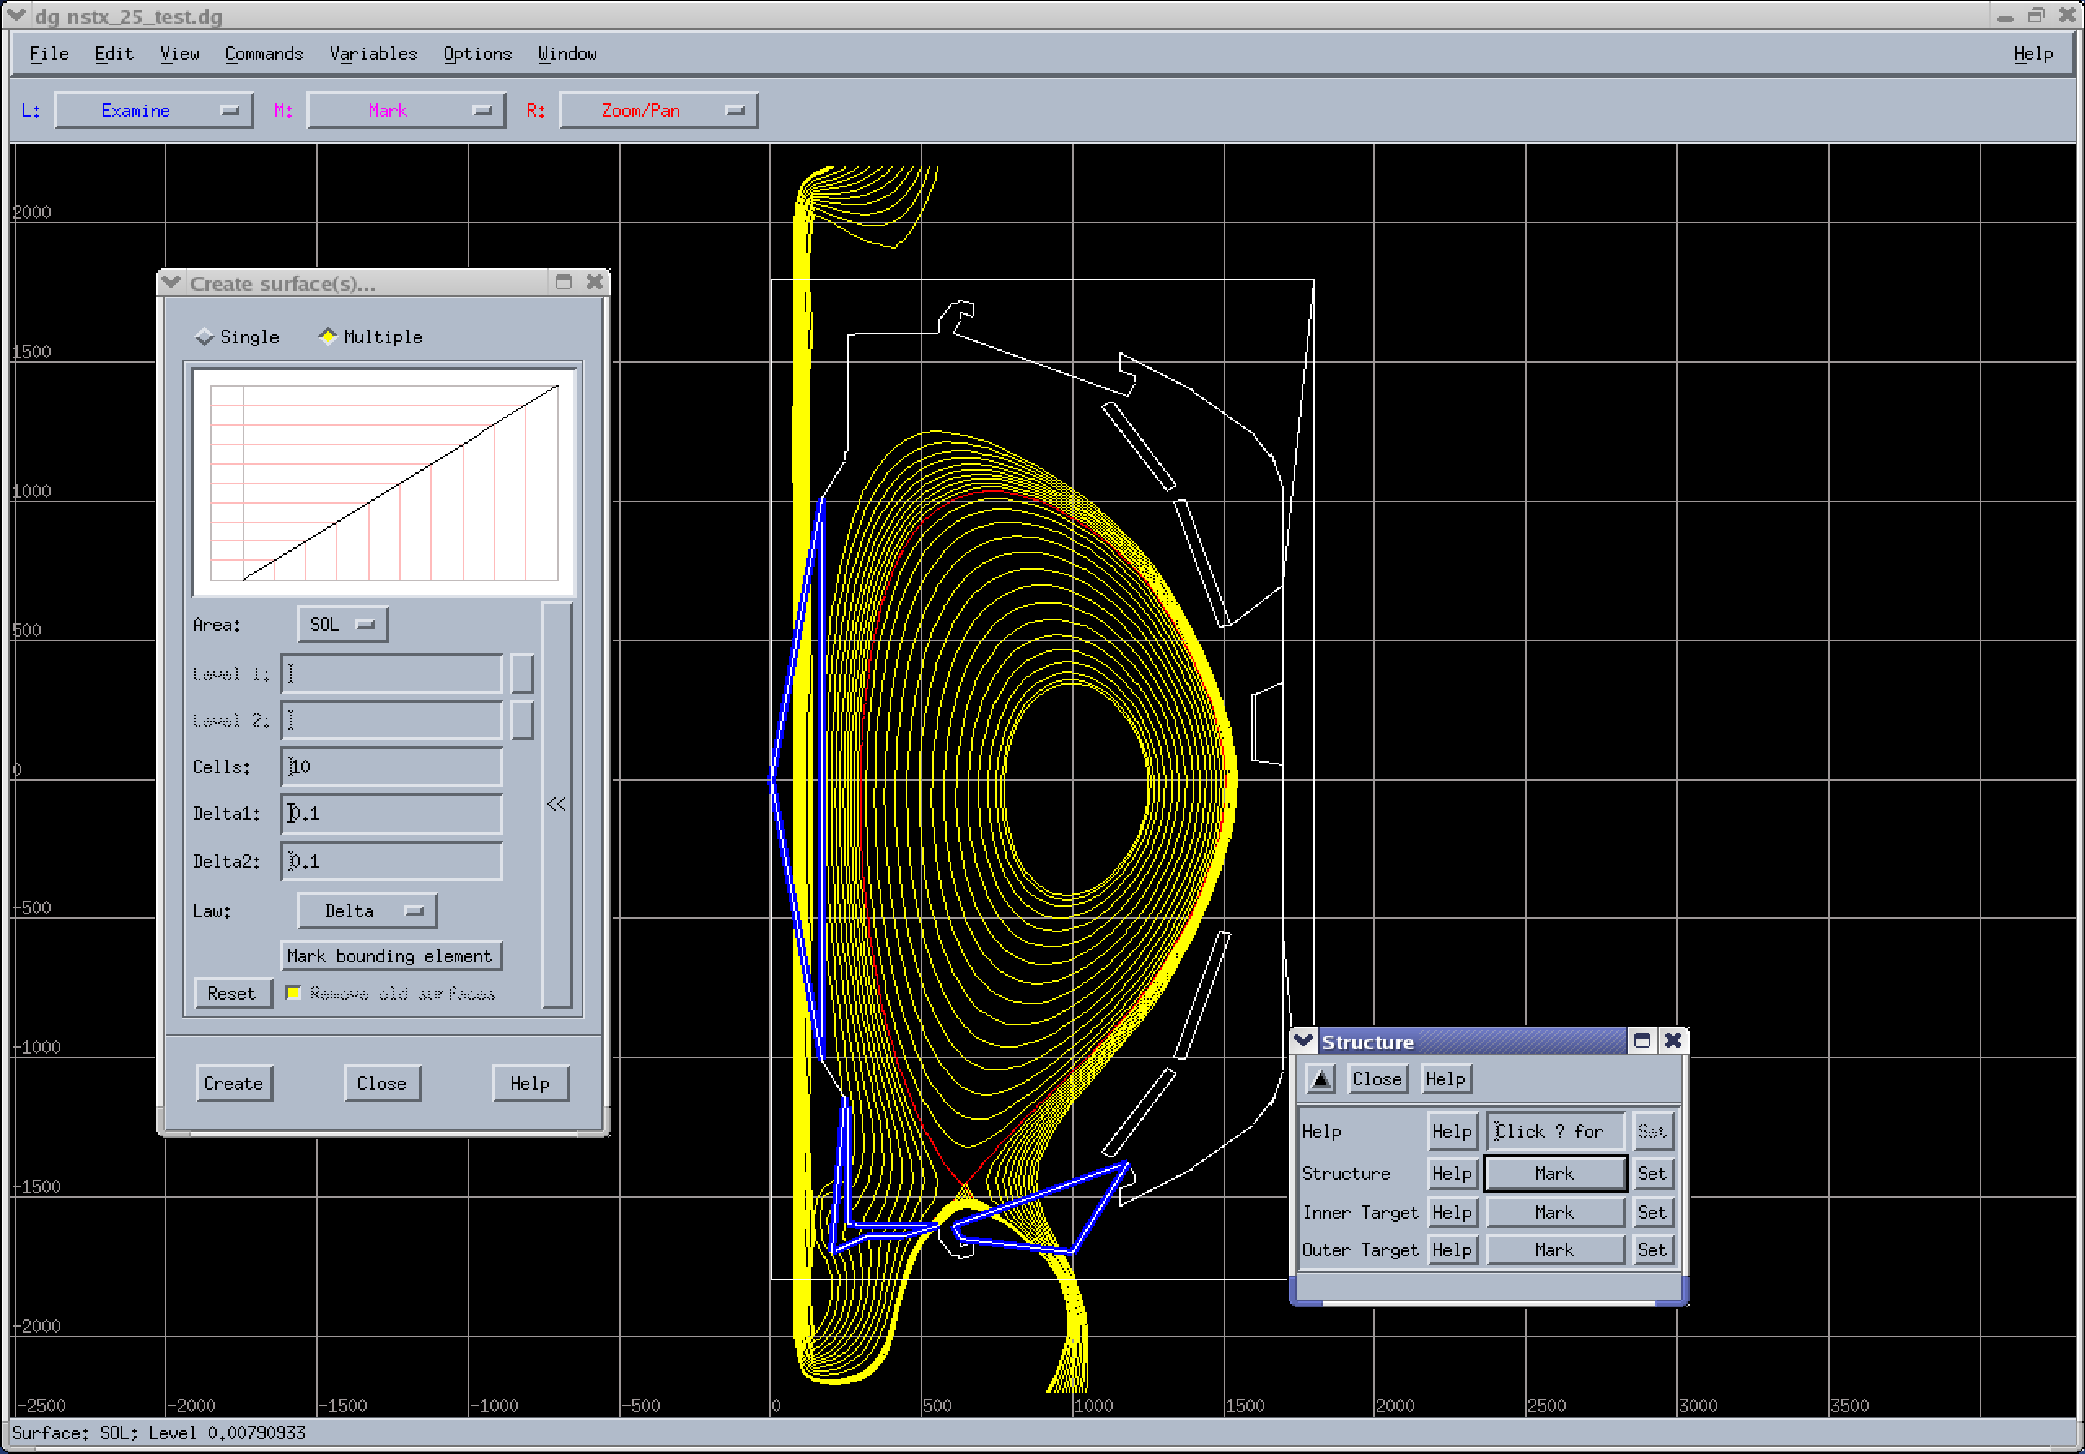
\includegraphics[width=15.0cm]{bde_structure.pdf}
\else
  
\includegraphics[width=15.0cm]{bde_structure.epsi}
\fi
\caption{\textbf{\texttt{Create Surface(s)...}} 
dialog with highlighted \textbf{\texttt{Structures}}.}
\label{createsurfacesfig}
\end{figure}

Note that the dialog will {\em not} enforce constraints on the number of
cells (e.g., that the number of core and PFR cells must be equal); the
user must check to be sure that all such constraints are satisfied.

DG's algorithm for calculating the outermost flux surface level for unbounded
regions (e.g., PFR and SOL)
uses the \textbf{\texttt{structure}} and 
\textbf{\texttt{inner / outer targets}} variables. The only
elements that the algorithm is aware of are those specified in the
\textbf{\texttt{structure}} variable, shown in Fig.~\ref{createsurfacesfig}.
Additionally, the algorithm
recognizes at least two subsets of the structures, the ``targets'', which
consist of all closed loops in the structure on which elements in the 
\textbf{\texttt{inner
target}} and \textbf{\texttt{outer target}} variables lie. 
All ``target'' elements must lie on a
closed loop in order that the targets have a well defined ``inside'' and
``outside''.
The outermost surface level is then defined as the flux value
differing most greatly from the value on the separatrix, whose corresponding
flux surface passes through every target but encounters no other elements in
the structure. This value is computed, to as much accuracy as the
resolution of the equilibrium allows, as the least of 1) the global maximum
on each target and 2) the global minimum on all other elements in the
structure, where maximum and minimum are understood to be in terms of
absolute deviation from the separatrix flux.

With this procedure, it is clear that the outermost level must be a flux
extremum of some element of the structure; we call this element the
``bounding element''. The capability was added to DG to record this bounding
element during surface creation and mark it from within the 
\textbf{\texttt{Create Surface(s)...}} dialog. See, e.g., Fig.~\ref{boundingelement}.
Note that the core region has no bounding
element. By
identifying what DG considers as the bounding element, we may easily adjust
the extent of the flux surfaces by moving the bounding element to change the
level of its extremum. Note that once the structure is
changed, the bounding element might different than before. 

\begin{figure}
\ifpdf
  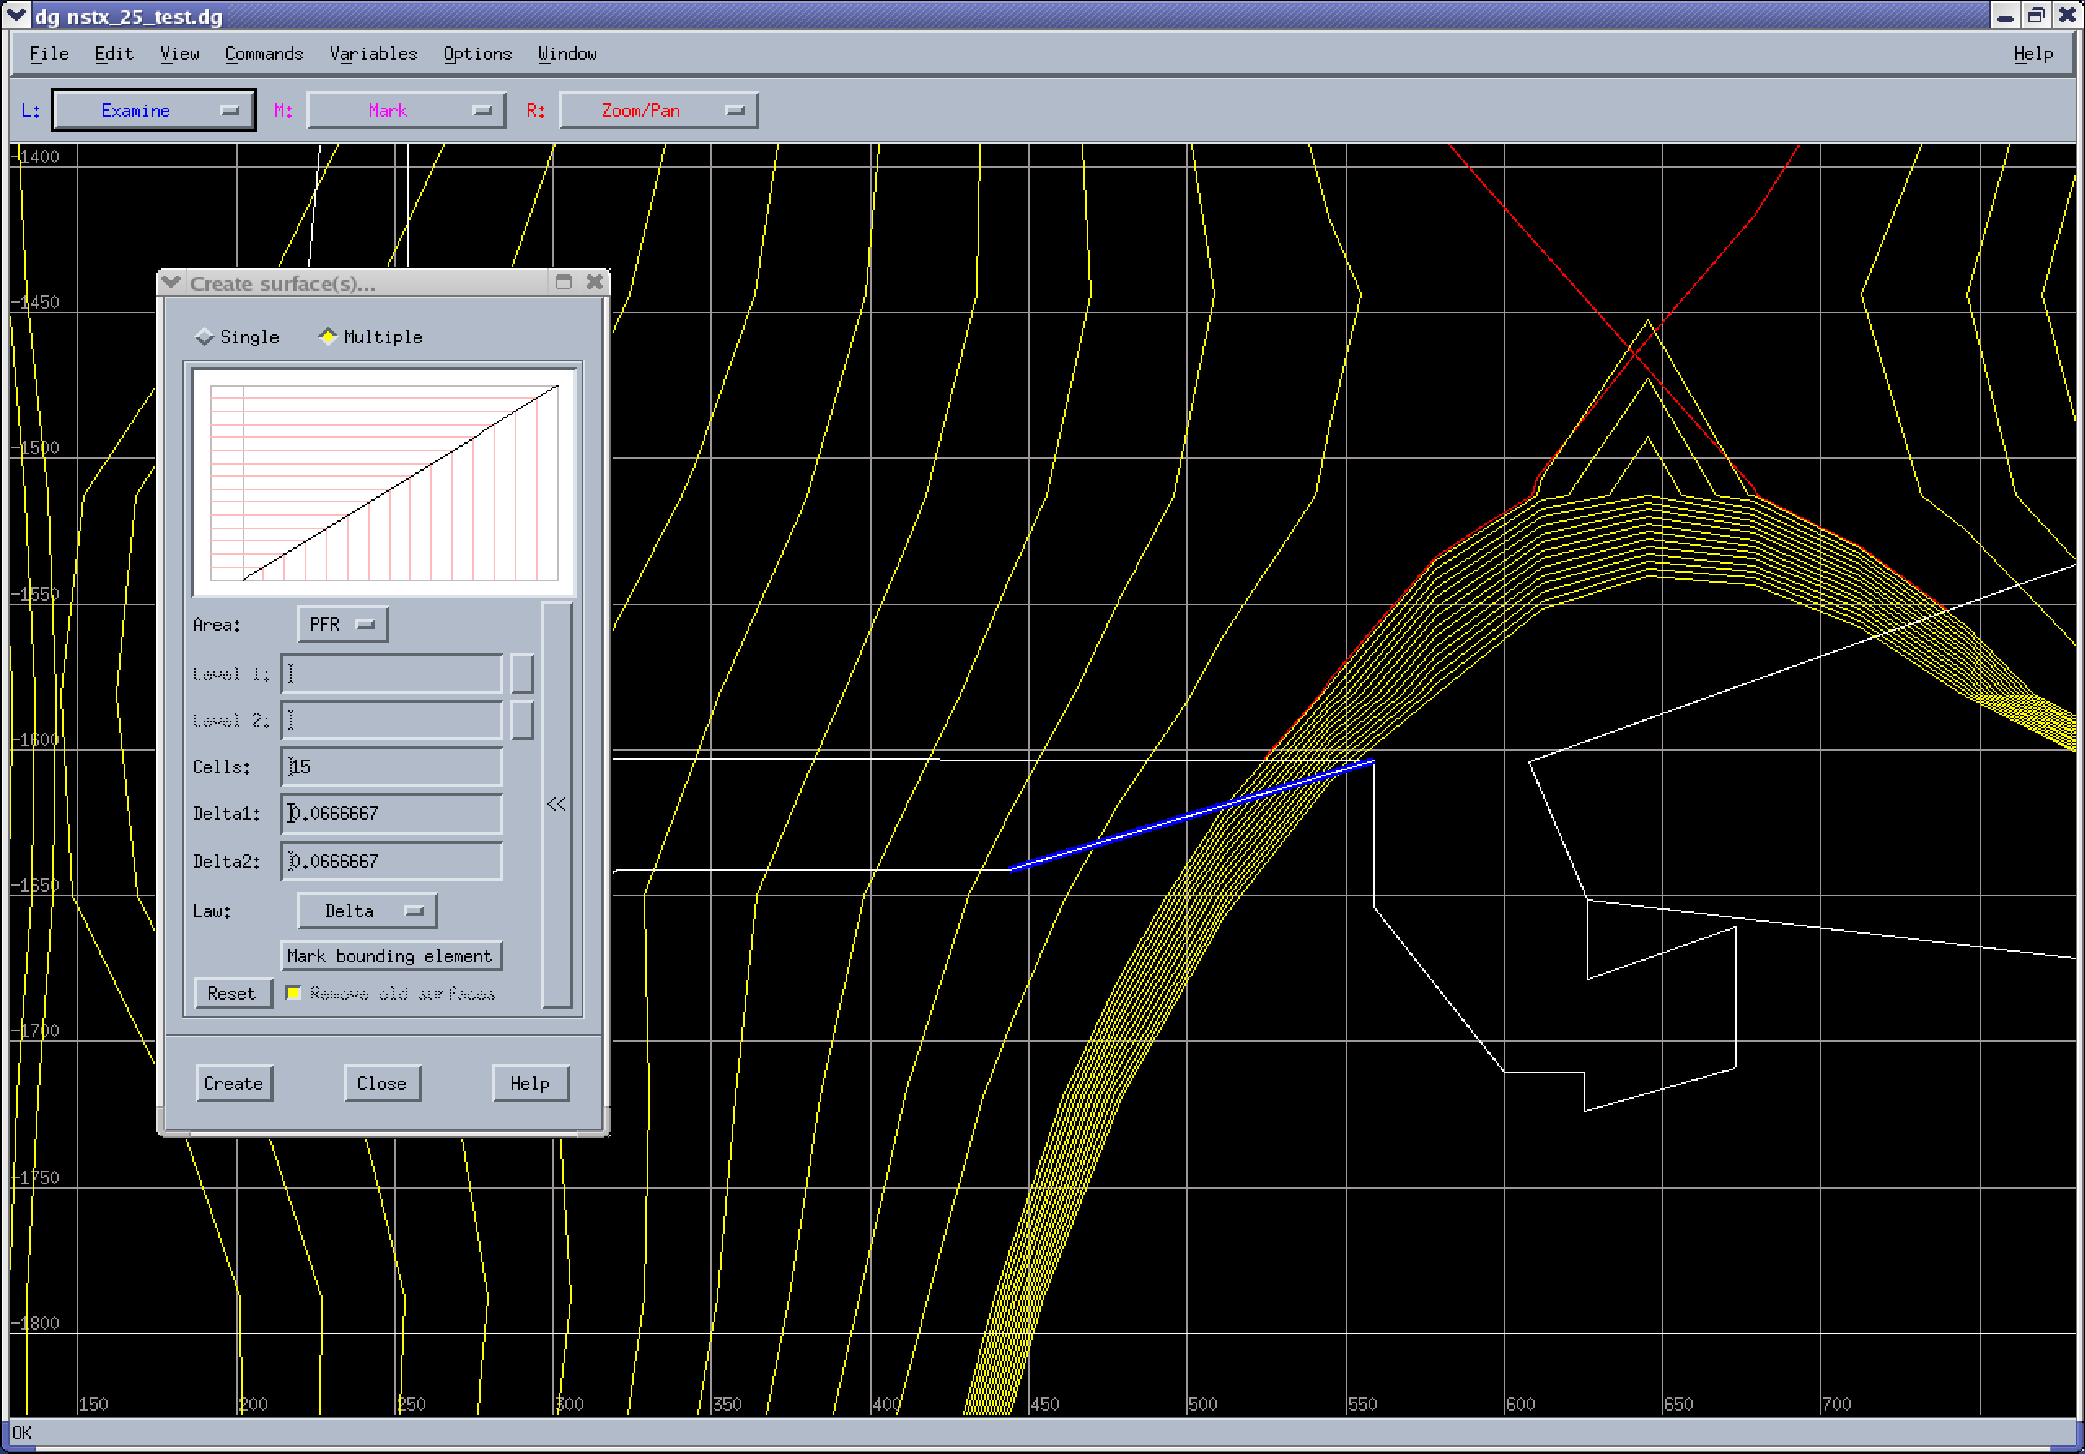
\includegraphics[width=15.0cm]{bde_pfr_zoom.pdf}
\else
  
\includegraphics[width=15.0cm]{bde_pfr_zoom.epsi}
\fi
\caption{Zoom of the PFR showing the highlighted ``bounding element''.}
\label{boundingelement}
\end{figure}

% \subsection{In case of difficulty \ldots}

% THIS DESCRIPTION STILL HAS A LITTLE TOO MUCH CODE JARGON (namely,
% the ``surface zones'') TO BE USEFUL.  Come back to this if it can
% be clarified.

% The process of creating surfaces is perhaps the most confusing and difficult
% aspect of using DG.  Moreover, the algorithm it uses for choosing the
% outermost flux surface level differs in detail from the one used by
% Carre.  If you are having problems getting the surfaces you want,
% you might benefit from reading the precise description of DG's
% current algorithm for setting the outermost flux level:

% \begin{itemize}
%   \item It is to be understood that ``maximum'' and ``minimum'' 
% always refer to the absolute flux deviation from the separatrix.
%   \item First, find the surface zone and the separatrix(ces) of the zone.  
% If
% there are two separatrices, draw surfaces from one to the other.  
% Else
% if the zone is marked as "limit by surface", find the farthest surface
% in the zone and draw surfaces to it.  (in practice, only one surface
% by be added manually in this zone, so that surfaces are always bounded
% by that one.)

% else, initialize the maximum level to infinity and get the structure
% variable, which includes the targets.  the structure is split into
% chains of adjacent elements, where each element in a chain may be
% connected to at most one other element at each endpoint.  if there are
% branching points in any chain, an error is returned.  the chains are
% organized into three groups: the first group consists of chains which
% contain elements that have been specified as a target.  these chains
% must contain the entire target variable and must form a closed loop,
% otherwise an error is returned.  the second group consists of chains
% with no target elements that form a closed loop, and the third group
% consists of chains with no target elements that do not form a closed
% loop.

% for each chain in the first group, for each element in the chain, if
% neither endpoint is in the surface zone, skip it, else get the maximum
% and minimum flux levels on the element from the equilibrium.  find the
% maximum level on the chain, and set the surface level maximum to the
% innermost of these levels.  also, find the minimum level on the chain,
% and set the surface level minimum to the outermost of these levels.

% for each of the elements in the second or third group, if the first
% endpoint is not in the surface zone, skip it, else get the minimum
% flux level on the element.  if it is less than the current surface
% level minimum, skip it, else if it is still less than the current
% surface level maximum, set the surface level maximum to this level.
% \end{itemize}


\section{Creating and editing grid points}

The \textit{\texttt{Add grid point}} tool lets you visually define
grid points. In addition, the
\textbf{\texttt{Edit  \begin{math}\vert{}\end{math}  Create  \begin{math}\vert{}\end{math}  Grid
point(s)}} menu command lets you define a grid point by specifying its
value or fill a zone on the separatrix with a given number of grid
points.  
In Carre mode, the only available method for creating grid points 
is with the ``multiple'' option of the 
\textbf{\texttt{Create grid point(s)\ldots}}
dialog box.  In particular, the \textit{\texttt{Add grid point}} tool
will not work, nor will the \textit{\texttt{Move}} or
\textit{\texttt{Delete}} tools have any
effect on the grid points.

In Carre mode, the operation of this dialog box is directly
analogous to that used to create surfaces (Sec.~\ref{createsurfaces}).
The ``zone'' refers to the section of the separatrix along which
grid points are to be created.
The number
of Cells must be input manually.  The line graph in the dialog box is a
simple depiction of the relative spacing of the grid points.  In Carre mode,
only the ``Delta Law'' is available.  In this case, the two parameters
``Delta1'' and ``Delta2'' specify a quadratic function used to determine
this spacing.  While these parameters can be input directly, the preferred
means of setting them is to click and drag the black line in the graph to
achieve the desired spacing variation.  When the ``Create'' button is
clicked, the grid points will be generated with this spacing and drawn in 
DG's main window.  If a model has an existing set of grid points that the
user wishes to tweak, click on one 
of these grid points with the \textit{\texttt{Examine}} tool and then
click the ``<<'' button in the \textbf{\texttt{Create grid point(s)...}} 
dialog; this will
import the parameters describing these grid points.
Note that the dialog will {\em not} enforce constraints on the number of
cells (e.g., that the number of grid points on either side of the
PFR must be equal); the
user must check to be sure that all such constraints are satisfied.

Use the
\textbf{\texttt{Edit  \begin{math}\vert{}\end{math}  Delete  \begin{math}\vert{}\end{math}  Grid
points}} menu command to delete all grid points.

\chapter{Working with chords}
\label{chords}

Chords are presently the only objects in DG that are not confined to the
poloidal plane (i.e., that may be non-axisymmetric).
For purposes of defining chords in three
dimensions, two coordinate
modes have been established. 
In ``Cartesian'' mode, $Z$ is the
vertical axis in the ``top-down view'' (Sec.~\ref{topdownview});
the horizontal axis in the poloidal plane is $X$ and the
vertical axis is $Y$ (note: this is a left-handed coordinate system).
In ``Cylindrical'' mode, $Z$ is the vertical coordinate in the poloidal
plane, identical to $Y$ in ``Cartesian'' mode. 
In the ``top-down view'',
the horizontal axis is
designated as $R$ and the toroidal angle as $\phi$ (counterclockwise relative
to the horizontal axis) is entered in degrees. 

Chords can be displayed with either 
\textbf{\texttt{View $\mid$ Display $\mid$ Chords}} or 
\textbf{\texttt{View $\mid$ Display $\mid$ 3dchords}}.  For chords
confined to the poloidal plane, these are identical, and chords will
not be visible in the ``top-down view''.  For chords with a toroidal
extent, selecting 
\textbf{\texttt{View $\mid$ Display $\mid$ Chords}} in the 
poloidal plane results in straight
line segments connecting the 
$X$ and $Y$ ``Cartesian'' coordinates of the chord end points.
Equivalently in the ``Cylindrical'' mode, these are the $R$
and $Z$ coordinates at the end points.  In contrast,
\textbf{\texttt{View $\mid$ Display $\mid$ 3dchords}} shows the projection
of the toroidal path of the chords on the $Z = 0$ (``Cartesian'')
or $\phi = 0$ (``Cylindrical'') plane.  In the ``top-down view'',
both \textbf{\texttt{View $\mid$ Display $\mid$ Chords}} and
\textbf{\texttt{View $\mid$ Display $\mid$ 3dchords}} show the straight
line paths of the chords in the $X$-$Z$ (``Cartesian'') or
$R \cos \phi$-$R \sin \phi$ (``Cylindrical'') plane.

Starting with file format version 115, chords with $X$, $Y$,
and $Z$
components may be saved and loaded.

\section{Creating chords}

The \textit{\texttt{Add Chord}} tool 
allows you to create chords graphically.  To
create a chord, move the mouse pointer to the desired location of its
beginning and press the mouse button the tool is assigned to. Without
releasing the mouse button, move the mouse pointer to the desired
location of the other end of the chord and release the mouse button.
``Chords'' can also be created from marked ``Elements'' via the 
\textbf{\texttt{Commands $\mid$ Convert $\mid$ Elements to chords}}
command.  Duplicate chords are not produced and the 
original elements are deleted.

The third method for creating chords is with the 
\textbf{\texttt{Edit $\mid$ Create $\mid$ Chord...}} dialog.

\section{Modifying chords}

The \textit{\texttt{Move}} tool allows chords to be manipulated in either
the poloidal plane or in ``top-down view''.  The user can
manipulate either the ``Chords'' object (displayed by
\textbf{\texttt{View $\mid$ Display $\mid$ Chords}}) or the
``3dchords'' object 
(displayed by \textbf{\texttt{View $\mid$ Display $\mid$ 3dchords}}.
The \textit{\texttt{Adjust chord}} tool moves an end point of the chord
while keeping its radial coordinate constant.  Holding down the
``shift'' key while using the \textit{\texttt{Move}} 
tool replicates this behavior,
but with slightly
different graphics that conform to the rest of the \textit{\texttt{Move}} 
tool.

Chords have an orientation, just like elements; this
orientation is displayed with 
\textbf{\texttt{View $\mid$ Display $\mid$ External normals}}.
The \textit{\texttt{Reverse normals}} tool can be used to change this 
orientation. Note that when this tool is dragged, it will only
operate on objects of the same type as the
first object encountered, either chords or elements. 

The \textit{\texttt{Extend chord}} tool linearly
extends (i.e., replaces) the second endpoint  of a chord to lie on
the nearest element, or the nearest marked element if elements have
been marked.  The
\textbf{\texttt{Edit $\mid$ Extend chords}} commands applies does
this for all marked chords.  The 
\textbf{\texttt{Edit $\mid$ Mark all chords}} command can be used
to mark all chords in preparation for extension.


{\em Note:} as of August 2007, the ``mathematically correct'' procedure
for extending chords has not been debugged. However, two macros
defined in \texttt{chords.c} may be used to select a different preferred
implementation of the procedure.  \texttt{EXTCHORD\_2D} 
selects the 2-D
procedure, which does not support chords with nonzero
toroidal extent,
and \texttt{EXTCHORD\_OLD} selects the partially correct, stable
3-D procedure, which does not work for horizontal chords and ignores
horizontal elements. (This is enabled in the current
release of DG).
If neither macro is defined, the code defaults to
the incomplete procedure, which may show unpredictable behavior during
use.

The \textbf{\texttt{Edit $\mid$ Delete $\mid$ Chords}} command
deletes all chords.

\chapter{Working with sources}

\section{Creating and editing sources}

DG allows the user to define sources and to attach variables to them.

To create sources, use the \textit{\texttt{Add source}} tool. Move the
mouse pointer to the desired location in the work area and press the
mouse button. A source will be created at this location. You can move
the mouse pointer to adjust its position. When finished, release the
mouse button.

To create a source by entering its coordinates, select
\textbf{\texttt{Edit  \begin{math}\vert{}\end{math}  Create  \begin{math}\vert{}\end{math}  Source...}}
. A dialog box will appear prompting for coordinates. Enter values and
press \textbf{\texttt{Create}}. A source will be created. The dialog
box will remain on the screen, allowing you to define multiple sources
without re-opening it. Press \textbf{\texttt{Cancel}} to close the
dialog box.

To move a source to a new location, use the
\textit{\texttt{Move}} tool. Select the source to move, drag it
to the new location and release the mouse button.

To delete a source, use the \textit{\texttt{Delete}} tool. Select the
source to delete and release the mouse button.

To delete all sources, issue the
\textbf{\texttt{Edit  \begin{math}\vert{}\end{math}  Delete  \begin{math}\vert{}\end{math} Sources}}
menu command.

\chapter{Working with meshes}

\section{Importing a SONNET format mesh}

DG allows you to import a mesh in the SONNET format.  Carre's output 
mesh can be converted into this format, as can meshes produced by other
codes.
The mesh will be 
displayed in the working area.

To import the mesh, use the
\textbf{\texttt{File $\mid$ Import $\mid$ Mesh...}} menu
command. A dialog box will appear prompting you for a filename. Select
a file from the list or type the filename in the edit field. Then press
\textbf{\texttt{Load}}. The mesh will be imported and displayed
in the work area. If nothing is displayed, select
\textbf{View  \begin{math}\vert{}\end{math} \texttt{ Picture view}} to
enlarge the area displayed. Also, make sure that
\textbf{\texttt{View $\mid$ Display $\mid$ Mesh}} is
enabled.

To hide or display the mesh, toggle
\textbf{\texttt{View $\mid$ Display $\mid$ Mesh}}
To unload the mesh, select
\textbf{\texttt{Edit $\mid$ Delete $\mid$ Mesh}}.

\section{Modifying a mesh}

DG's graphical interface permits limited modification of a mesh that has
been imported.  The altered mesh can be written out to a text file (in
the SONNET format) for use by other codes.  The primary tool for this
purpose is the ``Move mesh point'' tool.  The actions of this tool
are governed by the settings specified in the 
\textbf{\texttt{Options $\mid$ Mesh editing...}} dialog.
They only affect
one-dimensional movements of mesh
points.

``Slide along'' specifies how movements of mesh points are confined.
When ``Magnetic surfaces'' is in effect, the movement is confined to a
magnetic surface passing through the original location of the mesh
point. This method should work fine except for the vicinity of the 
X-point, where magnetic surfaces drawn by DG become distorted.
When ``Splines'' is in effect, the movement is confined to a spline
passing through a row of existing mesh points.  This method may be
useful in the vicinity of the X-point.

``Margin'' specifies the minimum distance between adjacent mesh
points. If this limit is about to get exceeded, adjacent points start
moving in order to ``make room''.
The ``Double border'' setting, when enabled, instructs DG to treat
outermost mesh cells as a double border. They would be resized
together with adjacent ``regular'' cells.

A modified mesh can be written out with the 
\textbf{\texttt{File $\mid$ Export $\mid$ Mesh...}} dialog.

\section{Repairing mesh cells using rotated
view and variable aspect ratio}

Mesh cells highlighted in pink in DG's main window are either concave
(have an interior angle greater than 180 degrees) or consist of
overlap with a neighboring cell.  These problems typically arise where
the mesh generator (Carre or otherwise) is forcing the mesh to
conform to the specified divertor target shape and usually involve
cells that are stretched significantly in one direction.

The ability to rotate and stretch the view allows the structure of the
problem cells to be discerned and repaired.
As an example, we consider a certain mesh generated for the NSTX experiment
which contains twisted cells near the inner divertor, Fig.~\ref{twisted}. 
By zooming, stretching, and rotating the view using the tools 
described in Secs.~\ref{rotateview} and \ref{stretchview}, 
we arrive at a much clearer depiction
of the problem, Fig.~\ref{twistedstretch}.
We see that the edges of the cells crossed the enforced boundary,
twisting the mesh cells in the process.  At this point, the user can
straightforwardly
use the \textit{\texttt{Move mesh point}} 
tool to manually repair the cells.

\begin{figure}
\ifpdf
  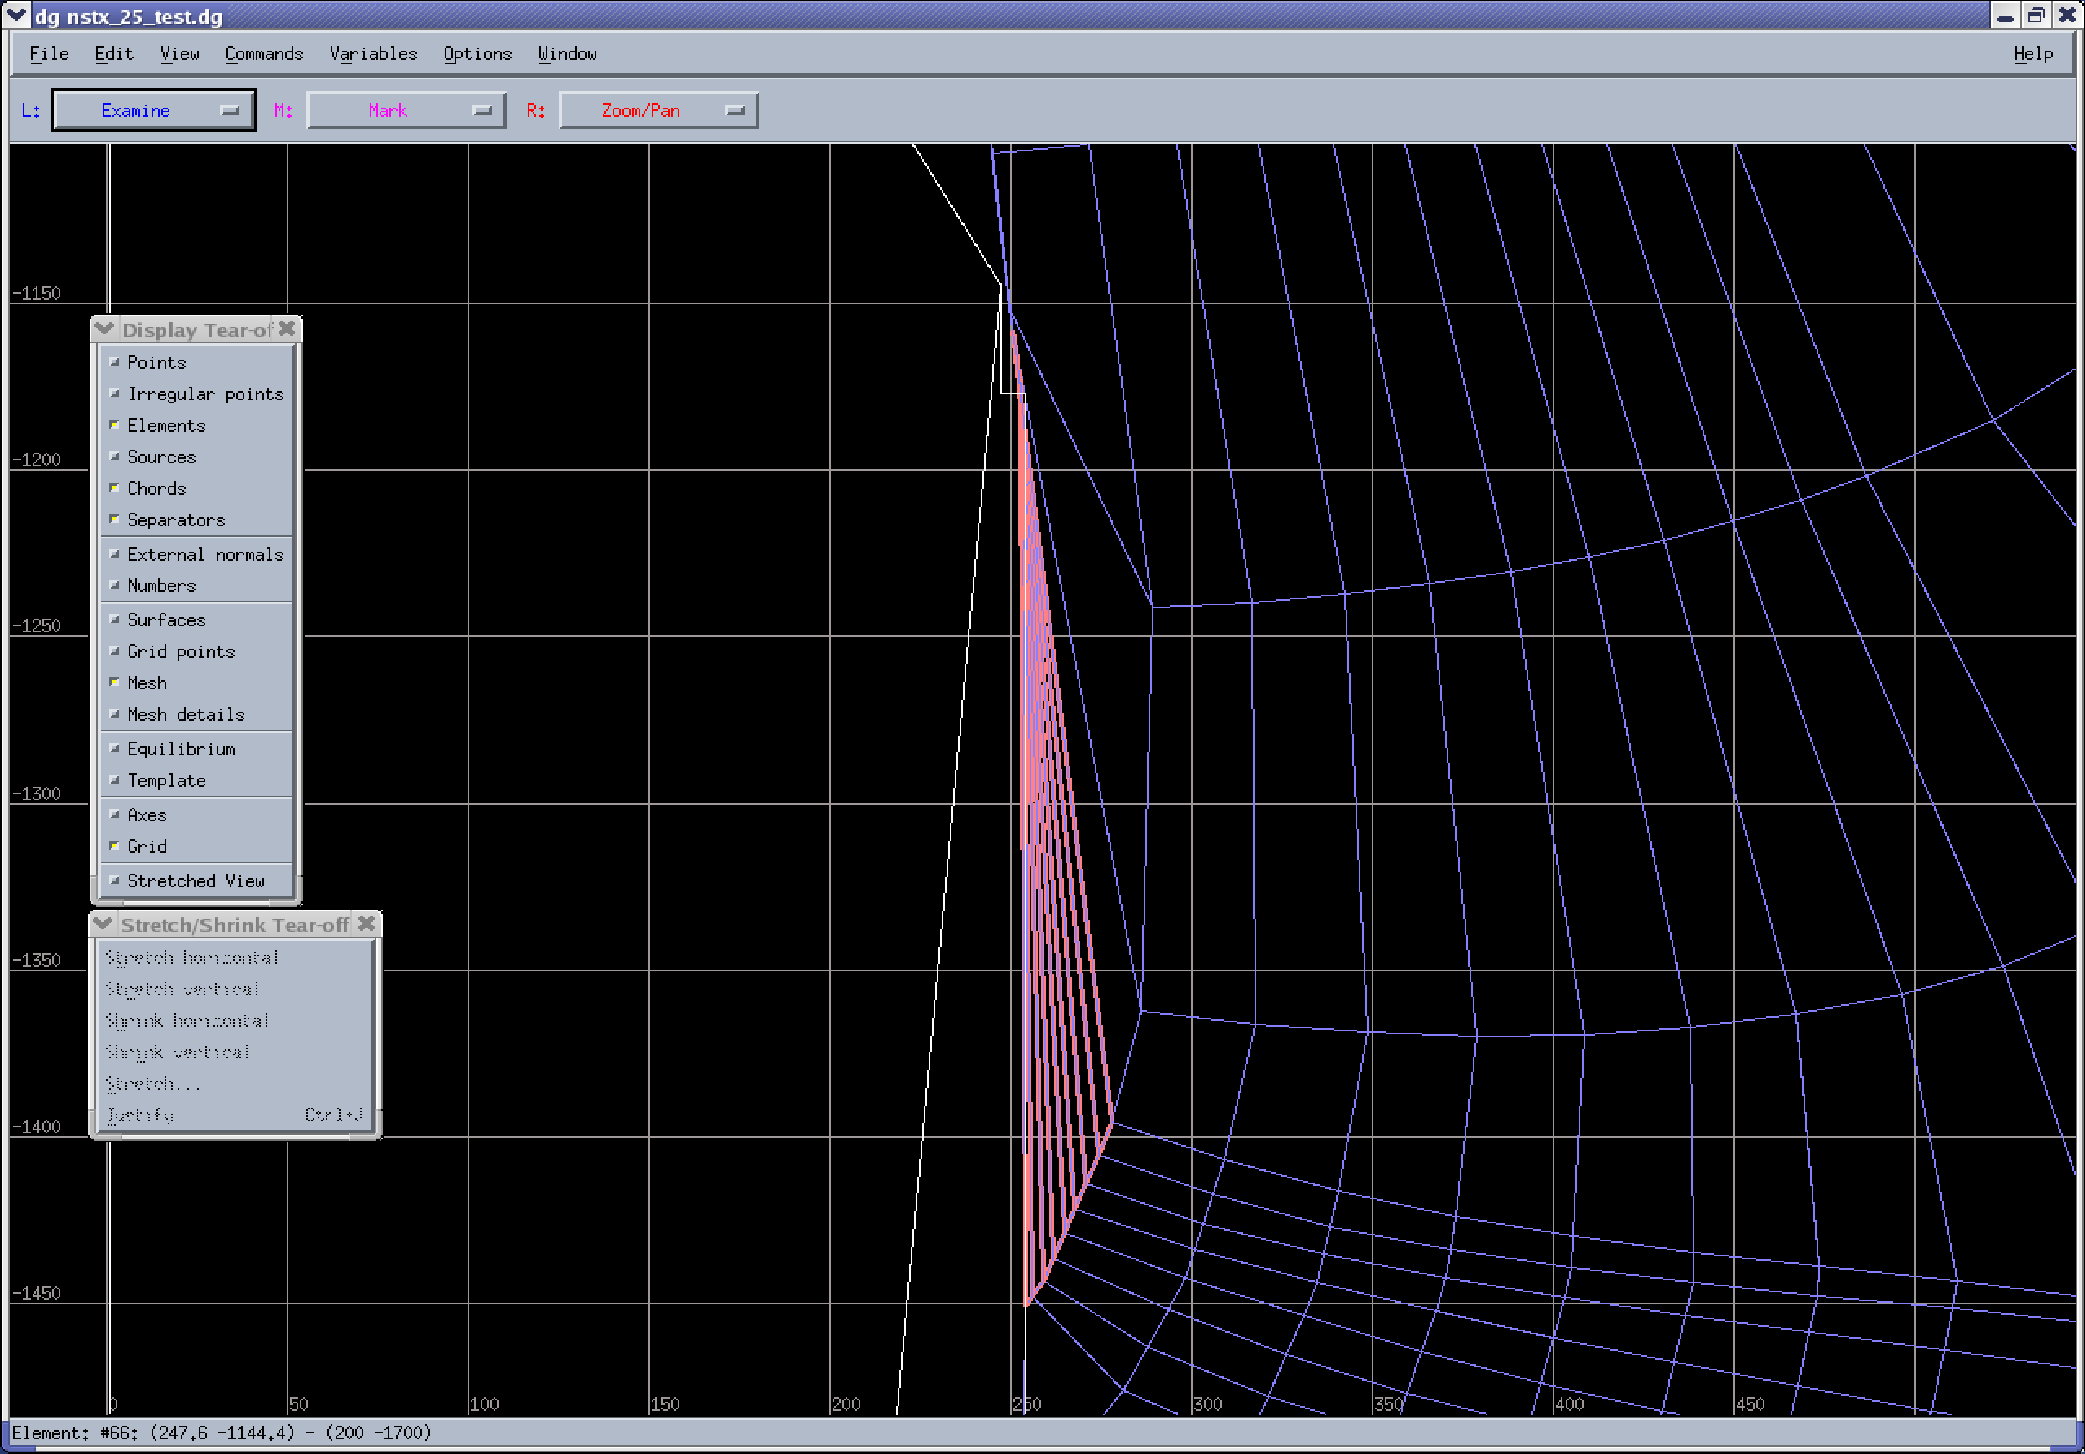
\includegraphics[width=15.0cm]{twisted_nostretch.pdf}
\else
  
\includegraphics[width=15.0cm]{twisted_nostretch.epsi}
\fi
\caption{Zoom of the twisted mesh cells near the inner divertor
target of an NSTX geometry.}
\label{twisted}
\end{figure}

\begin{figure}
\ifpdf
  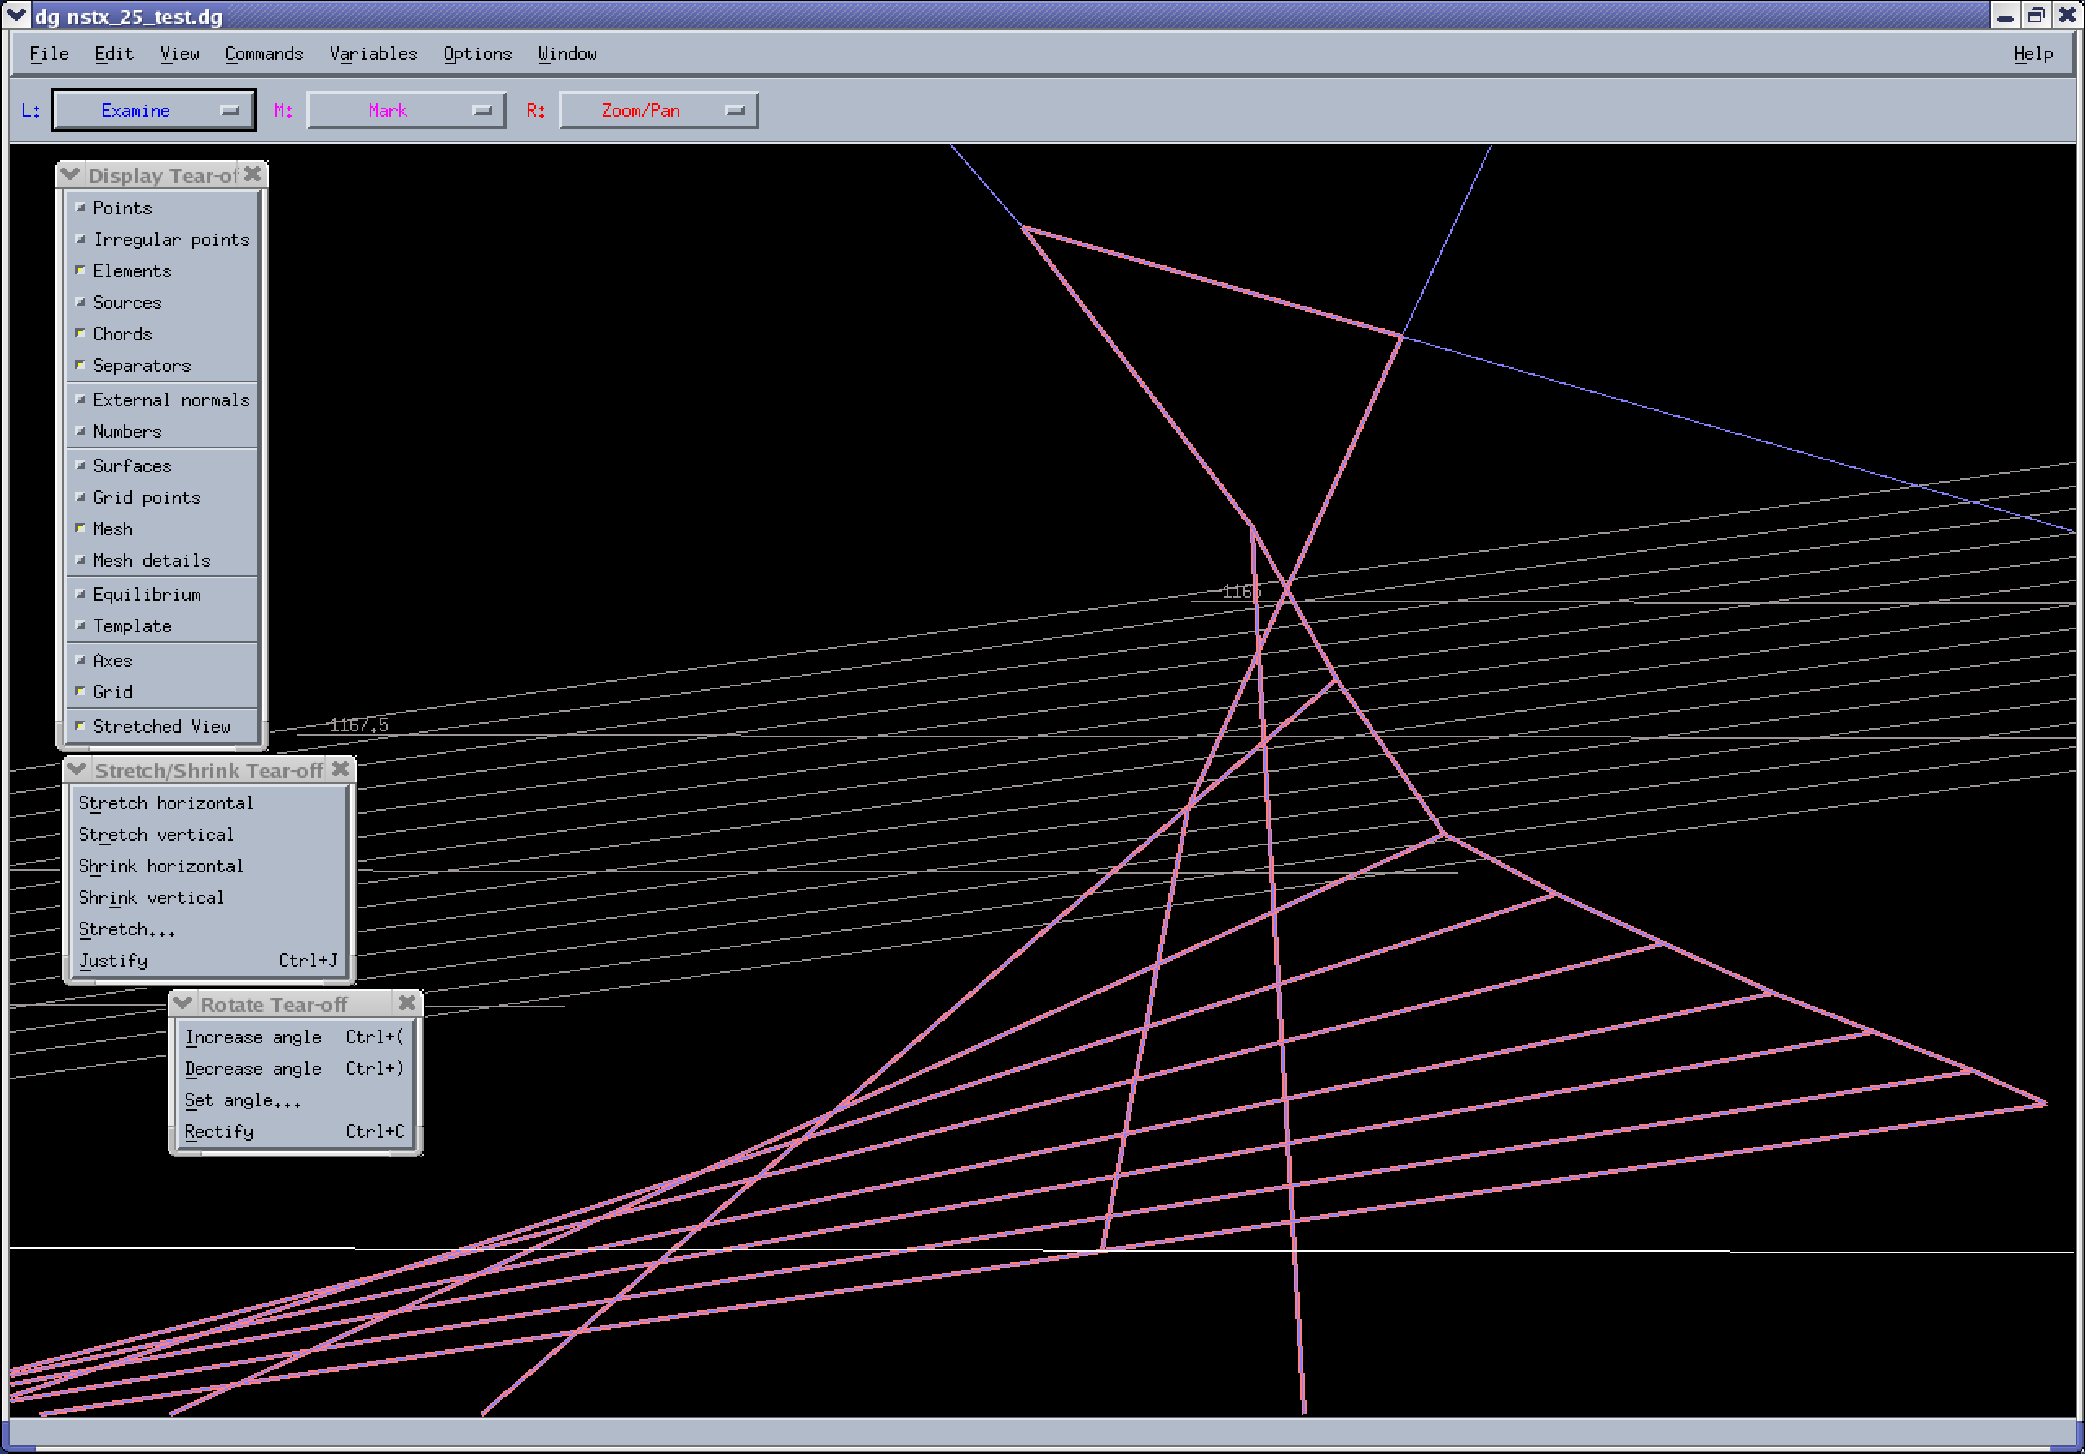
\includegraphics[width=15.0cm]{twisted_top_rotate_stretch.pdf}
\else
  
\includegraphics[width=15.0cm]{twisted_top_rotate_stretch.epsi}
\fi
\caption{After stretching and rotation, the overlapping of the cells in
the upper part of the region cells depicted in Fig.~\ref{twisted} becomes
clear.}
\label{twistedstretch}
\end{figure}



% \section{Defining cells}
% COMMENTED THIS OUT SINCE THERE ARE PRESENTLY NO SEPARATORS.

% With DG, you can define cells between the sonnet grid and the
% structure (both objects must be present). You define cells by creating
% separators between them. DG lets you create separators with the
% \textbf{\texttt{Edit \begin{math}\vert{}\end{math} Create \begin{math}\vert{}\end{math} Separators}}
% menu command. To adjust individual separators, use the
% \textbf{\texttt{Reposition tool}}. The
% \textbf{\texttt{Edit \begin{math}\vert{}\end{math} Delete \begin{math}\vert{}\end{math} Separators}}
% menu command removes all separators. You cannot add or remove
% individual separators with DG.

% To work with separators, you must define a suitable structure and
% import a sonnet grid.

% Use the
% \textbf{\texttt{Edit \begin{math}\vert{}\end{math} Create \begin{math}\vert{}\end{math} Separators}}
% menu command to create separators between the structure and the sonnet
% grid.

% Use the \textbf{\texttt{Reposition}} tool to attach a separator to a
% different structure point. Select the separator and move the mouse
% cursor a structure point. Then release the mouse button.

% Use the
% \textbf{\texttt{Edit \begin{math}\vert{}\end{math} Delete \begin{math}\vert{}\end{math} Separators}}
% menu command to delete all separators.

\chapter{Working with variables}

\section{Basics}

With DG, you can use ``Variables'' to specify information that cannot be
edited visually in the work area. Variables are written into the output
file and can be processed by other programs. Some variables (e.g., those
associated with \textbf{\texttt{targets}}
and \textbf{\texttt{structure}}) 
also have important functions in DG.  Variables are grouped
together into ``Layers''; each layer is visually represented
in the code as a dialog box in which the constituent variables can
be set, viewed, and modified.

Layers and their constituent variables must be defined  
by a power user before they can be instantiated and used
in a particular DG model. This
procedure is described in \textbf{\texttt{Customizing DG}}. Each
variable has following attributes:

\begin{description}
  \item[Name] is written into the output file and is
otherwise invisible.
  \item[Description] is the name that is shown to the user.
  \item[Type] defines type of values the variable can hold.
  \item[Scope] specifies what objects the variable applies
for.
  \item[Export/No export] determines whether values are
written into the output file.
  \item[Default value] is the default value for newly-created
objects.
  \item[Help text] is displayed to the user when s/he asks
for it.
\end{description}

These attributes are normally establised by a power user while defining
variables. A normal user should have some idea of the type and the scope
in order to be able to set correct values for correct objects.

Each variable has a \textbf{\texttt{type}}. A variable can hold either
a text value (\textbf{\texttt{integer}}, \textbf{\texttt{real}}, 
\textbf{\texttt{text}}, or \textbf{\texttt{filename}}) or a set of elements
(\textbf{\texttt{element}}, \textbf{\texttt{set of elements}},
\textbf{\texttt{target}}, \textbf{\texttt{structure}},
\textbf{\texttt{part of structure}}). DG prevents the user from
entering values of a wrong type.

The \textbf{\texttt{scope}} determines objects the variable is
attached to. There are 4 possible scopes:

\begin{description}
\item[Layers] means that the variable has one value for the
whole layer.
\item[Elements] means the variable has a separate value for
each element.
\item[Sources] means the variable has a separate value for
each source.
\item[Chords] means the variable has a separate value for
each chord.
\end{description}

As noted above, variables are organized 
into layers with DG displaying each
layer in a separate dialog box.

\section{Working with layers}

Layers may have one or more instantiations in a particular
model.  For some layers, a single instance is 
all that is needed 
to specify the desired information; DG will not
permit the creation of additional instances of this same
layer.  In the latter case, DG will assign an integer
count as the instances are created. 
Some layer instances are predefined (e.g., 
\textbf{\texttt{Structure}}) and cannot be created or destroyed
by the user, power or otherwise.

To create an instance of a specific layer, select the
layer from the
\textbf{\texttt{Variables  \begin{math}\vert{}\end{math}  Add}} submenu. A
dialog box for editing the variables in this layer
instance will
appear. If the maximum number of instances of a specific layer already
exist, this layer will not be displayed in the \textbf{\texttt{Add}}
menu. If this menu
becomes empty, the
\textbf{\texttt{Variables  \begin{math}\vert{}\end{math}  Add}} cascade
button will be grayed.

To destroy an instance of a layer, select its name in the
\textbf{\texttt{Variables  \begin{math}\vert{}\end{math}  Remove}} submenu.
If there are multiple instances of a layer, there will be a submenu associated
with that layer, listing the integer indices of those instances.
If only the minimum number of instances of a specific layer already exist,
layers of this type will not be displayed in this menu. If this menu
becomes empty, the
\textbf{\texttt{Variables \begin{math}\vert{}\end{math} Remove}} cascade
button will be grayed.

To display the dialog box for an existing layer instance, select its name 
and instance index (if applicable) under 
the \textbf{\texttt{Variables}} menu.

To hide the dialog box for a layer, press the \textbf{\texttt{Close}}
button in that dialog box.

\section{Setting variables}

The dialog box for each instance of a layer displays its variables,
allowing them to be set, viewed, and modified.
The title of this dialog box is the name of the layer; if there are 
multiple instances, the integer index of the particular index
is also displayed here.  At the top of the dialog
box, there is a row of buttons that affect the entire box.
Below this are fields for the individual variables.  Finally, there
is a status line at the bottom of the dialog box.

The ``$\bigtriangleup$'' 
button on top of the dialog box allows you to ``roll it up''
so that the box occupies less screen space. In
order to restore the dialog box to its full size, press this button
again.

The dialog box can be resized using the window manager. If it is
reduced in size, scrollbars appear, allowing you to scroll the
content. The functionality of the dialog box is NOT affected by
resizing it or rolling it up. In particular, the ``Set all'' button also
affects variables that are invisible.

For each variable, the dialog box contains its name, a ``Help'' button, a
text field for entering the new value (for text-like variables) or a 
``Mark''
button (for ``set of objects'' variables), and a ``Set'' button.
The ``Help'' button, when pressed, displays help about the variable.
The text field is used to enter new values for text variables. When
the text field has keyboard focus, the status line displays the
current value of the variable. For text variables that apply to
elements, chords or sources, only variables that apply to marked
objects are accessed.  ``Filename'' variables differ from ``Text''
in that the user can select the file interactively (press the
``Enter'' key on your keyboard in the text field to bring up the
file selection dialog); the variable is not valid unless the file 
exists and is readable at the time of the variable check.

The ``Mark'' button, available only for ``Set of objects'' variables,
marks the objects contained in the variable.
The ``Set'' button sets the variable to the new value. For text
variables, the new value must be entered in the text
field. For variables storing sets of objects, the objects must be
marked.

The ``Set all'' button in the top row, when pressed, has exactly the
same effect as pressing the ``Set'' button of each variable except that
empty new values for variables that apply to elements, sources or
chords are ignored. This button is only available if the layer
consists of text variables only.

The ``Reset all'' button, when pressed, resets all text fields to
present values of corresponding variables. It is only available in
layers consisting of text variables only. The text field is cleared
for variables that apply to elements, sources or chords when marked
objects have different values.

% NOT SURE THE HOLD BUTTON IS BEING USED.
% The "Hold" toggle button controls how text fields for variables that
% apply to elements, sources or chords are updated. When "Hold" is
% disabled, these fields are updated whenever an object is marked or
% unmarked. When "Hold" is enabled, these fields are not updated.

The ``Close'' button closes the dialog box.

Pressing the right mouse button over a text field or a button
associated with a variable brings up a pop-up menu. If the mouse has
less than 3 buttons, the menu can be displayed by pressing ``Ctrl+left''
button.
The ``Reset'' command sets the text field to the current value of the
variable, similar to the ``Reset all'' button but affecting only one
variable. For variables storing sets of objects, this command acts
exactly like the ``Mark'' button.
The ``Display values'' command displays values of variables that apply
to elements, chords or sources next to corresponding objects. In order
to remove these ``labels'', highlight any object or use the 
\textbf{\texttt{View $\mid$ Remove labels}} command from the main menu.
Commands in the ``Compare'' submenu compare values of the variable to
the value entered in the edit field and mark matching objects.
Both the ``Display values'' command and the ``Compare'' submenu are only
available for variables that apply to elements, sources or chords.


\chapter{Creating output files}

\section{Types of output files}

DG produces 3 output files:

\begin{description}
  \item[Structure file] contains the structure.
  \item[Targets file] contains targets, surfaces and grid
points.
  \item[Output file] contains elements, sources, separators
and the values of the variables associated with all of the
layer instances for the current model.
\end{description}

Current version of DG requires structure, targets, surfaces and grid
points to be defined. Also, all \textbf{\texttt{integer}} and
\textbf{\texttt{real}} variables must be set to non-empty values.

\section{Producing output files}

DG generates names of output files by attaching different extensions
to the name of the DG file. If the current file has no name yet, save
it with the \textbf{\texttt{File \begin{math}\vert{}\end{math} Save...}}
command before producing the output.

To produce the output files, choose the
\textbf{\texttt{File \begin{math}\vert{}\end{math} Output}} menu command.
A dialog box will appear asking for confirmation. Press
\textbf{\texttt{Ok }}to create the files.

\chapter{Customizing DG}

\section{Installing DG}

To install DG, you need to:
\begin{itemize}
  \item Compile and link its sources (additional 
guidance on how to do this with the version of DG 
distributed with DEGAS 2 are in Sec.~\ref{dgcompile}).
  \item Make sure that the help file exists and has the right name
  \item Make sure that the configuration file exists and has the right name
\end{itemize}

DG is an X Windows application. The correct \verb+DISPLAY+ setting is
necessary.

\section{Files needed by DG}

\begin{description}
  \item[dg] Executable file
  \item[dg.dgh] Help file
  \item[dg.dgc] Configuration file
\end{description}

\section{Specifying directory masks}

You can customize directory masks DG displays in file selection dialog
boxes by setting following environment variables:

\begin{description}
\item[\texttt{DGOPENMASK}] Directory mask for
\textbf{\texttt{File \begin{math}\vert{}\end{math} Open...}}
\item[\texttt{DGSAVEMASK}] Directory mask for
\textbf{\texttt{File \begin{math}\vert{}\end{math} Save...}}
\item[\texttt{DGEQUILMASK}] Directory mask for
\textbf{\texttt{File \begin{math}\vert{}\end{math} Equilibrium...}}
\item[\texttt{DGTEMPLATEMASK}] Directory mask for
\textbf{\texttt{File \begin{math}\vert{}\end{math} Template...}}
\item[\texttt{DGSONNETMASK}] Directory mask for
\textbf{\texttt{File \begin{math}\vert{}\end{math} Sonnet grid...}}
\end{description}

\section{The configuration file}

There is a special DG file, the \textbf{\texttt{configuration file}}.
Its filename is normally produced by appending \textbf{\texttt{.dgc}}
to the name of the executable. The configuration file has two
functions:
\begin{enumerate}
  \item When the \textbf{\texttt{File \begin{math}\vert{}\end{math} New}}
command is executed, the configuration file is loaded into the new
window.
  \item When a DG file is being opened, the configuration file is used to
update its definitions of variables and layers.
\end{enumerate}

DG normally writes these definitions in DG files. When a DG file is
opened, they are normally ignored and definitions from the
configuration file are used instead. This ensures that all files loaded
in DG have identical definitions of layers and variables.
Default values are not updated in the current version of DG.

\subsection{Specifying the configuration file}

Sometimes it is necessary to use a different configuration file or not
to use any at all.

To use a different configuration file, start DG with the following
command:
\begin{quote}
\textbf{\texttt{dg -cfg
 \begin{math}<\end{math} filename-with-extension \begin{math}>\end{math} }}
\end{quote}
To use DG without loading a configuration file, type
\begin{quote}
\textbf{\texttt{dg -nocfg}}
\end{quote}
NOTE: There are some bugs in DG that appear only when it is started
without any configuration and sometimes cause an exception.

\section{Creating or modifying the configuration file}

Use the \textbf{\texttt{Options \begin{math}\vert{}\end{math} Setup}}
menu to create or modify the configuration file.
Choose the \textbf{\texttt{Variables...}} submenu
in order to edit definitions of
variables and layers in the current file. The \textbf{\texttt{Layer
types}} dialog box will appear.

Press \textbf{\texttt{Save...}} to save the current file
as a configuration file. A dialog box will appear prompting for a
filename. Normally, it already contains the right name. Select
\textbf{\texttt{Ok}} to save the file in the current window as
configuration.
Press \textbf{\texttt{Close}} to close the dialog box.

\subsection{Adding, modifying and removing layer types}

To define a layer type, choose \textbf{\texttt{Add}} in the
\textbf{\texttt{Layer types}} dialog box. The new \textbf{\texttt{Layer
type options}} dialog box will appear.

Enter the name of the layer type to create in the
\textbf{\texttt{Name}} text field. The name should contain only
alphanumeric characters. This name will be written into the output
file.

Enter the description in the \textbf{\texttt{Description}} text field.
In the \textbf{\texttt{MinInstances}} / \textbf{\texttt{MaxInstances
text}} field, enter the minimum and the maximum number of layers of
this type. You will have to use 0 for \textbf{\texttt{MinInstances}}
because there are no layers of this type yet. You can change
\textbf{\texttt{MinInstances}} later after creating the minimum number
of layers.

Press the \textbf{\texttt{Ok}} button to create the layer type.

To remove a layer type, select it in the list and press
\textbf{\texttt{Delete}}.

To modify a layer type, select it in the list and press
\textbf{\texttt{Modify}}. The \textbf{\texttt{Layer type options}}
dialog box will appear. You can change name, description,
Min/MaxInstances here. Note that if you change the name, layers
contained in DG files under the old name will be ignored.

To close the \textbf{\texttt{Layer types}} dialog box, press
\textbf{\texttt{Close}}.

\subsection{Setting up variables}

To define the variables that will constitute a layer, first display its
\textbf{\texttt{Layer type:}} dialog box (``Modify''). This dialog
box contains a rectangular area with buttons. These buttons represent
row/column positions of variables in dialog boxes. Buttons containing
the string \textbf{\texttt{Empty}} mean no variable is defined at this
position.

To create a variable at a specific position, press the
\textbf{\texttt{Empty}} button at that position. The
\textbf{\texttt{New variable}} dialog box will appear.

Enter the name of the variable to be created in the \textbf{\texttt{Name}}
field. The name must contain only alphanumeric character.

Select the type and the scope in corresponding option menus. Check the
\textbf{\texttt{Do not export}} toggle button to prevent the variable
from being written into the output file. Structure and targets are
normally not exported because they are written into separate files.

Press \textbf{\texttt{Ok}} to create the variable.

To modify a variable definition, press its button in the
\textbf{\texttt{Layer type:}} dialog box. The
\textbf{\texttt{Variable:}} dialog box will appear. After making
changes, press \textbf{\texttt{Ok}}. Note that if you change the name,
variables contained in DG files under the old name will be ignored.

To remove a variable, press its button in the \textbf{\texttt{Layer
type:}} dialog box. The \textbf{\texttt{Variable:}}
dialog box will appear. Press \textbf{\texttt{Remove}} to remove the
variable.

\subsection{Adding help text to variables}

DG lets you add help text to variables. The user can display the help
text by pressing the \textbf{\texttt{Help}} button located near the name
of the variable in the \textbf{\texttt{Variables...}} dialog box.

To edit a help text for a variable, display its
\textbf{\texttt{Variable:}} dialog box and press
\textbf{\texttt{Edit help}}. The \textbf{\texttt{Help for variable}} dialog
box with a text editing field will appear. Edit the help text in
the editing field and press \textbf{\texttt{OK}}.

\subsection{Setting default values}

DG lets you define default values for variables. When a new layer,
element or source is created, the default values are used for the newly
created object.

It is suggested that you define default values for all variables
because DG will not generate output files when some variables have
empty values. A search for empty values can be very difficult and cost
a lot of time.


To define default values for variables in a layer type, display its
\textbf{\texttt{Layer:}} dialog box and
choose the variable for which you wish to set a default.
In its \textbf{\texttt{Variables:}} dialog box there is a
``Default value'' field for this purpose.

Default values from the configuration file are used only to create new
DG files. When opening an existing file, default values from the
configuration are ignored.

\section{Compiling DG for use with DEGAS 2}
\label{dgcompile}

\begin{enumerate}
  \item In the
\verb+degas2/dg_carre/DG/class+ directory, create a subdirectory
representing the particular experiment you will be working with,
e.g., \verb+mkdir nstx+, creating the DG ``nstx'' run directory.
  \item In \verb+degas2/dg_carre/class/nstx+ (or equivalent
for your situation), do: \verb+cp ../../dg .+, copying the DG
shell script to the run directory.
  \item In \verb+degas2/dg_carre+, type: 
\verb+source setup.csh nstx+ (or equivalent for your
situation).  This sets up pointers
to DG's ``nstx'' run directory.
   \item In \verb+degas2/dg_carre/mscl+, 
   \begin{enumerate}
        \item Create a run directory for the
specific type of computer being used (see the Makefile
for supported names), e.g., \verb+mkdir LINUX+,
        \item In that run directory, create a blank dependency file (to 
          temporarily fool the Makefile), e.g., 
\verb+touch dependencies.LINUX+,
        \item In the \verb+mscl directory+, do: 
\verb+gmake depend+.
        \item Then, \verb+gmake+.
        \item These are miscellaneous routines used by DG and Carre.
   \end{enumerate}
   \item In \verb+degas2/dg_carre/DG+,
   \begin{enumerate}
        \item Create a run directory, e.g., \verb+mkdir LINUX+,
        \item In the DG directory, do: \verb+gmake depend+.
        \item Then, \verb+gmake+.
        \item In the run directory, create a link to the help file. \\  
E.g.,
\verb+ln -s ../src/dg.dgh dg.dgh+
        \item Also in the run directory, create a link to the configuration
          file: \\
\verb+ln -s ../dg.dgc dg.dgc+
   \end{enumerate}
   \item In \verb+degas2/dg_carre/DG/equtrn+,
   \begin{enumerate}
        \item Create a run directory, e.g., \verb+mkdir LINUX+,
        \item In that run directory, create a blank dependency file (to 
          temporarily fool the Makefile), e.g., \verb+touch dependencies+,
        \item In the equtrn directory, do: \verb+gmake depend+.
        \item This will create \verb+.f+ (and perhaps \verb+.dbg+) 
files in the \verb+equtrn+ directory.  
These are not needed after this step and can be deleted.
        \item Then, \verb+gmake+.
        \item These routines are used to translate equilibrium data files from 
          one format to another (see Sec.~\ref{equtrn}).
   \end{enumerate}
   \item In \verb+degas2/dg_carre/Carre+,
   \begin{enumerate}
        \item Create a run directory, e.g., \verb+mkdir LINUX+,
        \item In that run directory, create a blank dependency file (to 
          temporarily fool the Makefile), e.g., 
\verb+touch dependencies.LINUX+,
        \item In the \verb+Carre+ directory, do: \verb+gmake depend+.
        \item Then, \verb+gmake+.
   \end{enumerate}
\end{enumerate}



\chapter{File formats}

\section{Simple template file format}

Besides the "Neutral File" exported from PATRAN, DG can also import
templates in a very simple format where the geometry is speified as a
set of polygons (in general, open). In this case, each line of the
input file either contains a pair of the co-ordinates of the next
corner, or is empty. 

\section{Structure file format}

The first line in the structure file contains the number of closed
chains in the structure.

Then, for each chain, starting with the outermost, the following block
appears:

\textbf{\texttt{ \begin{math}<\end{math}number of points in the
chain\begin{math}>\end{math} }}

\textbf{\texttt{ \begin{math}<\end{math}x1\begin{math}>\end{math}  ,
 \begin{math}<\end{math}y1\begin{math}>\end{math} }}

\textbf{\texttt{...}}

For the outermost chain, the bounding rectangle is added.

Points are output in counterclockwise order when the external normals
of the elements in the chain point outwards. Otherwise, they are output
in clockwise order.

\section{Targets file format}

The targets file (for a single null model) has the following format:

\textbf{\texttt{target 1}}

\textbf{\texttt{line}}

\textbf{\texttt{ \begin{math}<\end{math}x\begin{math}>\end{math} ,
 \begin{math}<\end{math}y\begin{math}>\end{math}}}

\textbf{\texttt{...}}

\textbf{\texttt{target 2}}

\textbf{\texttt{line}}

\textbf{\texttt{ \begin{math}<\end{math}x\begin{math}>\end{math} ,
 \begin{math}<\end{math}y\begin{math}>\end{math}}}

\textbf{\texttt{...}}

\textbf{\texttt{region 1}}

\textbf{\texttt{levels}}

\textbf{\texttt{ \begin{math}<\end{math}level\begin{math}>\end{math}}}


\textbf{\texttt{...}}

\textbf{\texttt{region 2}}

\textbf{\texttt{levels}}

\textbf{\texttt{ \begin{math}<\end{math}level\begin{math}>\end{math}}}

\textbf{\texttt{...}}

\textbf{\texttt{region 3}}

\textbf{\texttt{levels}}

\textbf{\texttt{ \begin{math}<\end{math}level\begin{math}>\end{math}}}

\textbf{\texttt{...}}

\textbf{\texttt{zone 1}}

\textbf{\texttt{points}}

\textbf{\texttt{ \begin{math}<\end{math}value\begin{math}>\end{math}}}

\textbf{\texttt{...}}

\textbf{\texttt{zone 2}}

\textbf{\texttt{points}}

\textbf{\texttt{\begin{math}<\end{math}value\begin{math}>\end{math}}}

\textbf{\texttt{...}}

\textbf{\texttt{zone 3}}

\textbf{\texttt{points}}

\textbf{\texttt{\begin{math}<\end{math}value\begin{math}>\end{math}}}

\textbf{\texttt{...}}

\textbf{\texttt{~}}

\textbf{\texttt{\begin{math}<\end{math}eof\begin{math}>\end{math}}}

The \textbf{\texttt{target1}} and \textbf{\texttt{target2}} blocks
contain point coordinates for targets.

The \textbf{\texttt{region}} \textbf{\texttt{1...3}} blocks contain
levels of surfaces. Regions have following meaning:
\begin{description}
  \item[region 1] Main Plasma
  \item[region 2] SOL
  \item[region 3] Private Flux
\end{description}

The \textbf{\texttt{zone 1...3}} blocks contain values of grid points
(between 0 and 1). Zones have following meaning:
\begin{description}
  \item[zone 1] Main chamber
  \item[zone 2] Inner divertor
  \item[zone 3] Outer divertor
\end{description}

\section{Output file format}

The output file has the following format:

\textbf{\texttt{userdata}}


\textbf{\texttt{p1}}


\textbf{\texttt{\begin{math}<\end{math}x\begin{math}>\end{math} ,
\begin{math}<\end{math}y\begin{math}>\end{math} ,
\begin{math}<\end{math}z\begin{math}>\end{math}}}

\textbf{\texttt{...}}


\textbf{\texttt{p2}}

\textbf{\texttt{\begin{math}<\end{math}x\begin{math}>\end{math} ,
\begin{math}<\end{math}y\begin{math}>\end{math} ,
\begin{math}<\end{math}z\begin{math}>\end{math}}}


\textbf{\texttt{misselem}}

\textbf{\texttt{\begin{math}<\end{math}number\begin{math}>\end{math}}}

\textbf{\texttt{...}}

\textbf{\texttt{sprtrs}}

\textbf{\texttt{\begin{math}<\end{math}number\begin{math}>\end{math}}}

\textbf{\texttt{...}}

\textbf{\texttt{chords}}

\textbf{\texttt{\begin{math}<\end{math}xs\begin{math}>\end{math} ,
\begin{math}<\end{math}ys\begin{math}>\end{math} ,
\begin{math}<\end{math}xe\begin{math}>\end{math} ,
\begin{math}<\end{math}ye\begin{math}>\end{math}}}

\textbf{\texttt{sources}}

\textbf{\texttt{\begin{math}<\end{math}x\begin{math}>\end{math} ,
\begin{math}<\end{math}y\begin{math}>\end{math}}}

\textbf{\texttt{\begin{math}<\end{math}layer
name\begin{math}>\end{math} \begin{math}<\end{math}layer
instance number\begin{math}>\end{math}}}

\textbf{\texttt{\begin{math}<\end{math}variable\begin{math}>\end{math}}}

\textbf{\texttt{...}}


\textbf{\texttt{...}}


\textbf{\texttt{finish}}

\textbf{\texttt{p1}} and \textbf{\texttt{p2}} sections contain the
coordinates of the origins and the ends of elements (respectively), 
ordered by element number. For unused element 
numbers, dummy coordinates are output.
The $Z$ coordinate is always 0.

The\textbf{\texttt{ misselem}} section contains unused element
numbers. Elements with these numbers \textbf{\texttt{must}} be ignored.

The \textbf{\texttt{sprtrs}} section lists numbers of separators in
\textbf{\texttt{p1}} and \textbf{\texttt{p2}} arrays (currently
disabled so that this section will be empty).

The \textbf{\texttt{chords}} section lists the $X$, $Y$ coordinates
of the start (``s'') and end (``e'') point of each chord.  Note
that the $Z$ coordinate is {\em not} listed so that chords with
a toroidal extent (see Sec.~\ref{chords}) are {\em not} properly described.

The \textbf{\texttt{sources}} section lists sources.

For each layer, a \textbf{\texttt{\begin{math}<\end{math}layer
name\begin{math}>\end{math} \begin{math}<\end{math}layer
instance number\begin{math}>\end{math}}} section is present. Layer name is the
name of the layer. Layer instance number is used to distinguish between
layers of the same type. Each section contains a
\textbf{\texttt{\begin{math}<\end{math}variable\begin{math}>\end{math}}}
entry for each variable in the layer.

The
\textbf{\texttt{\begin{math}<\end{math}variable\begin{math}>\end{math}}}
block has following formats:
\begin{itemize}
  \item Text variables that apply to the layer:
\textbf{\texttt{\begin{math}<\end{math}variable
name\begin{math}>\end{math}
\begin{math}<\end{math}value\begin{math}>\end{math}}}
  \item Text variables that apply to elements or sources:
\begin{quote}
\textbf{\texttt{\begin{math}<\end{math}variable
name\begin{math}>\end{math}}}

\textbf{\texttt{\begin{math}<\end{math}value\begin{math}>\end{math}}}

\textbf{\texttt{...}}
\end{quote}
  \item For variables that apply to elements, a value for each element number
is included. Dummy values are used for unused numbers. For variables
that apply to sources, a value for each source is included. Values are
written in the same order as sources in the \textbf{\texttt{sources}}
section.
  \item ``Set of elements'' variables that apply to the layer:
\begin{quote}
\textbf{\texttt{\begin{math}<\end{math}variable
name\begin{math}>\end{math}}}

\textbf{\texttt{\begin{math}<\end{math}element
number\begin{math}>\end{math}}}

\textbf{\texttt{...}}
\end{quote}
\end{itemize}
\end{document}
